\chapter{Un Islam Français est possible}

\begin{marginfigure}
\centering

\includegraphics[width=0.91222in,height=0.54469in]{ImageIslamFrance/media/image6.png}
\caption{
Normalien, agrégé de géographie, \textbf{Hakim El Karoui} a enseigné à
l'université Lyon II avant de rejoindre le cabinet du Premier ministre
en 2002, où il était chargé de ses discours. Après un passage à Bercy,
il rejoint, en 2006, la banque Rothschild où, avec Lionel Zinsou, il
anime la practice Afrique. En 2011, il rejoint le cabinet de conseil en
stratégie Roland Berger où il est co-responsable de l'Afrique et du
conseil au gouvernement français. En 2016, il fonde sa propre société de
conseil stratégique Volentia. Hakim El Karoui est aussi essayiste (il a
publié trois livres chez Flammarion qui traitent de questions
économiques et géopolitiques) et entrepreneur social (il a créé le club
du XXIe siècle, les Young Mediterranean Leaders et est avec Bariza
Khiari à l'origine de « l'appel des 41 », paru le 31 juillet 2016 dans
le JDD). L'analyse des données de l'enquête inédite, réalisée dans le cadre de ce
rapport, a été effectuée par \textbf{Antoine Jardin}, docteur en science
politique et ingénieur de recherche au CNRS.
A noter, une polémique : \href{http://www.observatoire-des-sondages.org/musulmans-de-france-quand-la-fausse-monnaie-chasse-la-bonne}{La fausse monnaie chasse la bonne} qui souligne des biais classiques de sondage sur données sensibles mais les solutions (en particulier interrogation en présentiel) ne me paraissent pas très pertinentes.}
\end{marginfigure}



\subsection{Avant-Propos}


Pourquoi travailler sur l'islam en 2016 ? Parce que la violence qui
s'est déchaînée en son nom en France, contre des Français, ne peut
rester sans réponse. Il faut engager des changements profonds dans
l'organisation de cette religion pour lui donner les moyens de lutter
contre le fondamentalisme religieux qui crée un terreau favorable au
terrorisme. Pourquoi travailler sur l'islam en cette pré-campagne
électorale ? Parce que l'on ne peut se satisfaire des sempiternelles
polémiques sur l'inscription des signes d'appartenance islamique dans
l'espace public, -- le burkini étant le dernier exemple\ldots-- comme
seules réponses politiques au djihadisme et au fondamentalisme : tout
cela traduit surtout un sentiment d'impuissance et nourrit crispations
et angoisses au sein de la société française.

Ces peurs sont renforcées par la méconnaissance générale des musulmans
français : qui sont-ils ? Quels rapports entretiennent-ils avec la
religion ? Avec les autorités religieuses ? Les rares connaissances dont
nous disposons étaient imprécises et ne se fondaient que sur des
estimations. C'est pour porter remède à cette situation que l'Institut
Montaigne a conduit avec l'IFOP une enquête inédite, soumise à la plus
grande rigueur méthodologique et au strict respect de la législation en
vigueur. \paragraph{Que nous enseigne l'IFOP ?} Que le nombre de musulmans en France
est moins important que ne l'avancent bon nombre de chiffres
fantaisistes : ils représentent 5,5 \% de la population de plus de 15
ans en métropole. Que cette population est nettement plus jeune que la
moyenne nationale. Qu'elle est aussi moins qualifiée, même si une classe
moyenne et une élite émergent clairement. Cette large enquête atteste
également qu'une majorité des musulmans de France a un système de valeur
et une pratique religieuse qui s'insèrent sans heurts majeurs dans le
corpus républicain et national. Elle montre enfin que nombreux -- mais
minoritaires -- sont les -- jeunes -- Français de confession musulmane,
qui se définissent d'abord et avant tout par leur identité religieuse,
suivant une logique implacable : 
\begin{quote}
    « plus vous êtes fondamentaliste, plus
vous êtes musulman et donc plus vous êtes vous-même ».
\end{quote} En arrière-plan,
une relation complexe avec la France, l'attrait du fondamentalisme
religieux étant un moyen pour eux d'exprimer une forme de révolte contre
une société qui les rejette ; c'est du moins très largement leur
perception. Malgré les difficultés à comparer les évolutions dans le
temps, en raison de la rareté des chiffres disponibles et des
contraintes méthodologiques, il ne fait pas de doute que cette tendance
est en augmentation sensible depuis dix ans.

Deux réalités très différentes donc : une majorité silencieuse, très
souvent pratiquante mais sans conflit majeur avec les normes de la
société française, d'une part ; une minorité, attirée par le
fondamentalisme, qui utilise l'islam pour dire sa révolte, d'autre part. On peut le déplorer, s'en féliciter, vouloir le
combattre ou le respecter, ce fait social est bien réel. Il faut le
traiter, dans le contexte qui est le nôtre - celui d'une violence
terroriste et sans limite perpétrée au nom de l'islam, qui rend
angoissant pour une majorité de Français le mouvement d'affirmation
identitaro-religieux voire théologico-politique qui est à l'œuvre.

Or, le système mis en place en 2003 avec la création du Conseil français
du culte musulman (CFCM) a montré ses limites :


\begin{itemize}
\item
  (i) influence des États étrangers à qui la France a sous-traité une
  forme de contrôle social et sécuritaire ;
\item
  (ii) incompréhension face aux mutations d'un islam de plus en plus
  identitaire, porté par des jeunes garçons et des jeunes filles, très
  souvent Français de naissance, que ne comprennent pas les responsables
  des institutions actuelles -- quasiment tous des hommes, souvent âgés
  de plus de 60 ans, nés à l'étranger ;
\item
  (iii) incapacité, enfin, à intervenir face au phénomène rampant de la
  radicalisation religieuse alors que théories du complot, antisémitisme
  et postures victimaires fleurissent chez ceux-là même qui trouvent
  dans un islam autoritaire -- voire radical -- un moyen d'affirmation.
\end{itemize}


De nombreux problèmes ont fait obstacle, jusqu'à présent, et ont entravé
les évolutions de l'organisation de l'islam en France :


\begin{itemize}
\item
  géopolitiques, d'abord, car l'organisation de l'islam de France se
  trouve enchâssée dans l'écheveau complexe des relations de la France
  avec les pays du Maghreb et la Turquie ;
\item
  organisationnels, ensuite, parce que, malgré les inquiétudes relatives
  au communautarisme musulman, la « communauté musulmane en France »
  n'existe tout simplement pas : ni sentiment d'appartenance, ni
  intérêts communs identifiés, ni capacité d'action groupée. Depuis
  trente ans, les ministres de l'Intérieur successifs ont d'ailleurs
  tous échoué à trouver un interlocuteur représentatif ;
\item
  financiers également, car malgré certains financements venus de pays
  étrangers « amis » (le Maroc, la Turquie, l'Algérie et l'Arabie Saoudite), l'islam est sous-financé et pâtit, par ailleurs, d'un manque de transparence qui
entrave sa capacité à collecter les dons des fidèles et qui est dommageable pour sa réputation ;
\item
  institutionnels, enfin, car il faut que le gouvernement français fasse
  bien davantage confiance aux musulmans de France et notamment aux
  élites qui ont émergé ou sont en train de le faire. À cet égard, la
  nomination de Jean-Pierre Chevènement à la tête de la Fondation pour
  l'islam de France n'est pas un signe encourageant et elle a suscité,
  malgré les qualités de cet ancien Ministre, incompréhension et
  déception. Il ne serait sans doute venu à l'esprit de personne de le
  désigner pour une telle mission auprès des autres grandes religions
  présentes sur le sol national.
\end{itemize}


Cinq mutations majeures doivent pourtant être engagées :


\begin{itemize}
\item
  « sortir l'islam de France de la minorité » en comprenant enfin que
  les musulmans ne sont ni des mineurs qu'il faut mettre sous tutelle ni
  des irresponsables toujours divisés qu'il faut considérer avec
  commisération sans jamais les croire capables d'agir efficacement :
  cela a été souvent l'attitude des pouvoirs publics, confrontés il est
  vrai à des querelles incessantes de représentants plus ou moins auto-
  proclamés de l'islam en France. Cet objectif repose sur deux
  impératifs :

  \begin{itemize}
  \item
    mettre fin à la tutelle - longtemps acceptée voire encouragée par la
    France - d'États étrangers, qui ne tolèreraient en aucune manière
    sur leur sol ce qu'ils pratiquent en France : imagine-t-on la
    France, ou l'Italie qui vit sous régime concordataire, financer le
    culte catholique dans tel ou tel pays musulman et le cabinet du
    Premier ministre envoyer le texte des prêches chaque dimanche aux
    desservants français établis dans ces pays ? C'est pourtant ce qui
    se passe en France aujourd'hui. Cette action sera réussie quand les
    flux financiers venus de ces pays ne seront plus dirigés vers « leur
    » communauté, mais de façon claire et transparente, vers une
    organisation reconnue dont les moyens financiers seront destinés à
    l'ensemble des musulmans de France, quelle que soit leur origine ;
  \item
    faire émerger de nouveaux cadres, religieux et laïcs, nés en France,
    soucieux de prendre en main une communauté embryonnaire et de
    répondre aux très nombreux défis auxquels sont confrontés les
    musulmans de France. La solution pour y parvenir, c'est de leur
    donner une légitimité institutionnelle en les associant à la
    création et à la gouvernance de la Fondation pour l'islam de France
    et à l'association musulmane pour un islam de France ;
  \end{itemize}

\item
  assurer à l'islam de France des ressources financières transparentes,
  destinées à un usage collectif, afin de structurer une véritable
  organisation de l'islam, de salarier les imams et de répondre au fait
  social indéniable que constitue « la nouvelle fierté islamique » de
  nombreux musulmans de France, qui font de l'islam un objet moins
  religieux qu'identitaire. La solution, c'est une redevance sur le
  halal et des institutions reconnues capables d'attirer des dons;
\item
  travailler de façon efficace à la formulation et à la diffusion
  d'interprétations de l'islam alternatives aux discours de fermeture,
  de séparation et de soumission;
\item
  contribuer, autant que le permet la loi de 1905, à la lutte contre le
  discours fondamentaliste, notamment \emph{via} le financement de la
  formation -- culturelle - et du travail des aumôniers dans tous les
  lieux fermés (écoles, prisons, armées, établissements hospitaliers,
  etc.) et \emph{via} l'enseignement de l'arabe à l'école publique (dans
  un contexte où cet enseignement se diffuse très rapidement dans les
  mosquées et les écoles coraniques, du fait, notamment, de l'absence
  d'offre de formation à l'école) ;
\item
  une réflexion doit, enfin, être engagée sur l'absence de l'islam du
  concordat qui régit encore la relation entre les cultes et l'État en
  Alsace-Moselle. Il en va de l'égalité entre les citoyens et de la
  capacité de l'État de créer une faculté de théologie capable de
  travailler rapidement sur des interprétations religieuses en phase
  avec la réalité française contemporaine ;
\item
  lever les ambiguïtés qui pèsent sur certaines pratiques locales (baux
  emphytéotiques, carrés confessionnels, garanties d'emprunt) pour
  garantir aux musulmans que ces pratiques juridiques sont conformes à
  la Constitution.
\end{itemize}


Pour y arriver, il faut tenir compte de la nouvelle réalité de l'islam
dans notre pays : les musulmans sont majoritairement nés en France et
aujourd'hui Français pour les trois-quarts d'entre eux. Autre évolution
sociologique importante : si les ouvriers, les employés et les chômeurs
sont surreprésentés par rapport à la moyenne nationale, une nouvelle
élite bien formée et bien insérée dans le monde professionnel est en
train d'émerger.

Construire un islam français est donc possible mais, ô combien difficile
! Il faudra assumer, parfois, la crispation des uns et des autres et
avoir suffisamment bien préparé ces évolutions afin qu'elles puissent
aboutir. Il faudra se préparer à répondre
aux polémiques venues de tous les camps tant cette question est
sensible, complexe et sujette à manipulation en ces temps de campagne
électorale. Il faudra être prêt à bousculer les conservatismes et les
idées reçues de toutes parts.

C'est pourquoi l'État devra s'investir au plus haut niveau pour faire
émerger cette nouvelle organisation de l'islam français, car il a encore
un rôle à jouer pour faciliter les changements avant de se retirer
ensuite, conformément au principe de laïcité. L'enjeu est essentiel :
c'est notre cohésion nationale qu'il faut préserver, et, c'est aussi,
pour les musulmans, l'occasion d'inventer une nouvelle modernité
religieuse.


\subsubsection{Un portrait des musulmans de France}

Voir des Français -- chrétiens, musulmans, juifs, athées -- mourir « au
nom de l'islam » : cette réalité est devenue la nôtre depuis les
attentats perpétrés par Mohamed Merah en 2012. Les événements de ces
deux dernières années, violents, terribles, différents par leurs cibles,
leur envergure mais pas par les réactions qu'ils ont suscitées, se
nouent les uns aux autres dans une déflagration sordide. La peur et la
haine dominent. Les esprits, notamment politiques, sont troublés et
confus : le piège tendu par les djihadistes -- attiser la haine contre
tous les musulmans pour encourager ces derniers à les rejoindre -- reste
ouvert, béant. Avec le risque qu'un jour il ne se referme sur la société
française.

Une brève analyse des couvertures des principaux magazines
hebdomadaires1 montre que l'islam est invariablement présenté comme
porteur de violence et de haine : il s'agit là exactement de ce que
veulent les djihadistes qui, par leurs actions, orientent cette
couverture médiatique. Une quarantaine de numéros des six magazines les
plus vendus en France ont ainsi placé un sujet lié à l'islam en
couverture au cours des douze derniers mois ; en moyenne, chaque
semaine, un magazine a dédié sa « une » à l'islam. La rhétorique
visuelle de ces numéros recourt d'ailleurs souvent aux mêmes éléments :
sur un fond sombre s'accumulent des photos d'hommes en armes, de leaders
enturbannés, de sabres ; larges polices, couleurs vives, contrastent
avec des fonds sombres. Le champ lexical des enquêtes policières est
mobilisé : il faut trouver les \emph{« complices »}, les \emph{«
cerveaux »}, les

\emph{« armées souterraines »}. Lorsqu'il s'agit d'étudier les relations
de l'État et de l'islam, le champ lexical est celui de la défaite, de la
faiblesse. Les « unes » portant sur des régimes se revendiquant de
l'islam (l'Iran ou l'Arabie Saoudite) utilisent le vocabulaire de la
menace et de la peur. Une tonalité commune se dessine dans le traitement
de ces sujets, dont les champs lexicaux et les visuels sont ceux de la
menace, de l'alarme et de l'inquiétude. L'islam reste à déchiffrer. Les
enjeux géopolitiques et les courants extrémistes accaparent la
représentation. Il convient de remarquer qu'un seul numéro sur ces
quarante s'intéresse au quotidien des musulmans français\sn{\emph{M le magazine du Monde,} « La religion, la mode, le travail, les
garçons, paroles de jeunes filles voilées », 21/05/2016.}.


Cette tendance a commencé avec la révolution islamique en Iran qui a
inauguré l'âge des revendications politiques entremêlées de référents
religieux. Depuis les années 1980, les crises survenues en Palestine, en
Jordanie, au Liban, en Irak, en Algérie, en Bosnie, en Afghanistan, en
Tchétchénie, en Syrie, en Libye et au Yémen sont peu à peu devenues «
islamiques ». Les « printemps arabes » et leurs conséquences, la montée
de l'islam politique, sont venus confirmer que tout sujet concernant des
pays de population musulmane pouvait désormais donner lieu à une lecture
par le prisme du religieux.

Depuis la fin des années 1980, la France débat de l'islam et de son
rapport avec la République et la laïcité. Le premier débat portait sur
le voile en 1989, suivi par ceux de 1993 et de 2003. Avant les
commentaires sur la présence ou non d'une composante musulmane dans
l'imaginaire des émeutes des banlieues en automne 2005, qui ont précédé
les discussions sur l'identité nationale, alimentées par
l'interprétation des propos de tel ou tel intellectuel musulman, les
saillies de représentants d'ONG salafistes sur les plateaux de
télévision, les prêches d'imams radicaux, etc. L'islam ne semble exister
que dans trois cadres: les relations internationales et géopolitiques ;
les attentats terroristes et les faits de société liés à la montée du
salafisme ou de l'islamisme politique ; ainsi que leur relation avec les
valeurs laïques.

Face au danger terroriste, l'État se doit d'apporter une réponse
sécuritaire. C'est évidemment légitime mais cela ne peut être suffisant.
Il faut également répondre par la connaissance aux défis que les
événements de 2015 et de 2016 ont fait naître, afin d'éclairer les
débats à venir d'éléments solides et objectifs. On bute alors sur la
méconnaissance de la population musulmane française : qui sont-ils ? Que
pensent-ils ? Nul ne le sait vraiment en raison des carences de la
statistique publique dès lors qu'il s'agit de religion4. Pourtant, des
enquêtes d'opinion sont légales et possibles. C'est pourquoi nous avons
lancé une grande enquête d'opinion sur les musulmans de France. Les
objectifs sont simples : il faut mieux les connaître, afin d'être à même
ensuite de proposer des solutions susceptibles d'accélérer la sereine
insertion de la majorité silencieuse, mais aussi des mesures destinées à
combattre le fondamentalisme, tout en ramenant le plus grand nombre
possible de musulmans -- souvent des jeunes -- tentés par l'intégrisme
vers des croyances et des idées en phase avec les valeurs républicaines.


 
\section{L'islam Français} 
\subsection{Les écoles}
Les écoles confessionnelles musulmanes en France Paysage de
l'enseignement confessionnel en France


Il existe deux types d'établissements scolaires privés en France : les
établissements sous contrat et ceux hors contrat.

\textbf{Les établissements sous contrat} constituent la majorité des
établissements scolaires privés. Après cinq années d'exercice, un
établissement d'enseignement privé hors contrat peut demander à être lié
à l'État par un contrat. Ce contrat oblige l'établissement à accueillir
les enfants sans distinction d'origine, d'opinion ou de croyance. En
contrepartie, l'État assure la rémunération des enseignants, qui sont
tenus d'avoir réussi des concours analogues à ceux de l'enseignement
public, et les collectivités publiques financent le fonctionnement de
l'établissement, dans les mêmes proportions que celui des écoles et des
établissements publics. La France compte 7 845 établissements sous
contrat (primaire et secondaire confondus), dont 7 300 établissements
catholiques, une centaine d'établissements juifs, 34 établissements
protestants et seulement six établissements musulmans. Environ 16 \% des
élèves scolarisés en France le sont dans des établissements privés sous
contrat.

L'ouverture des \textbf{établissements hors contrat} est uniquement
soumise à une déclaration préalable auprès du procureur de la
République, du préfet et du recteur ainsi que du maire pour les
établissements primaires87. On estime leur nombre à

1 300 mais seulement plus de 300 sont des établissements confessionnels
:

200 établissements catholiques, une cinquantaine d'établissements juifs,
une quarantaine d'établissements protestants et une cinquantaine
d'établissements musulmans. 61 370 élèves sont scolarisés dans des
établissements hors contrat, selon les chiffres de l'année 2015-2016,
soit moins de 0,5 \% de l'ensemble des élèves scolarisés en France88. Si
elles sont minoritaires, les écoles hors contrat ont vu leur nombre
augmenter de 26 \% entre 2011 et 2014, selon le ministère de l'Éducation
nationale. 16 établissements confessionnels musulmans ont ainsi été
créés en 2015, principalement des écoles primaires89.

\subsection{Situation de l'enseignement confessionnel musulman}

L'enseignement confessionnel musulman est un phénomène minoritaire, mais
qui se développe ces dernières années. Constituée en 2014, sous
l'impulsion de l'UOIF, la Fédération nationale de l'enseignement
musulman (FNEM) réunit 56 établissements et entend à la fois organiser
et représenter l'enseignement confessionnel musulman.

Selon les chiffres 2015-2016 de la FNEM, on dénombre :


\begin{itemize}
\item
  \textbf{5 000 élèves scolarisés dans l'enseignement privé musulman,}
  dont 3 050 écoliers, 1 280 collégiens et 670 lycéens ;
\item
  \textbf{56 unités pédagogiques,} dont 35 écoles, 14 collèges et sept
  lycées ; accueillant chacun une centaine d'élèves en moyenne ;
\end{itemize}

\begin{itemize}
\item
  \textbf{Seulement deux établissements sont sous contrat d'association
  avec l'État et quatre sous contrat d'association
  partielle}90\textbf{.} Les 50 autres établissements adhérents à la
  FNEM sont hors-contrat.
\end{itemize}


\subsection{Les relations entre l'État et l'islam en Europe : une institutionnalisation à parfaire}

\paragraph{Relations entre l'État et les religions dans 15 pays européens}

La conception de la présence musulmane européenne par les États
européens est désormais mue par une double volonté
d'institutionnalisation et de co-administration de l'islam en Europe ;
et ce afin de contenir les franges radicales, de rassurer l'opinion
publique et de prendre acte de la pérennité de cette présence. La
volonté de créer les conditions institutionnelles dépasse la simple
reconnaissance du culte musulman et vise à développer un islam européen
idiosyncratique.

Cette évolution s'est accompagnée d'un changement de paradigme
institutionnel, profondément marqué depuis les années 2000 par
\textbf{deux tendances lourdes :}


\begin{itemize}
\item
  les difficultés éprouvées par les musulmans européens pour
  s'organiser, auxquelles s'ajoute un déficit de légitimité auprès des
  musulmans ;
\item
  la succession d'attentats terroristes commis par des musulmans
  européens sur le sol européen.
\end{itemize}

Trois remarques liminaires sur l'institutionnalisation :


De prime abord, il est intéressant de relever que les divers conseils
européens \textbf{représentatifs prétendent représenter l'islam et non
les musulmans.} Cette nuance est loin d'être anodine, au sens où les
diverses puissances publiques ne pouvaient qu'accompagner
l'institutionnalisation du culte et non la constitution d'un « lobby »
musulman, qui serait le porte-voix des revendications, des desiderata ou
des intérêts politiques des musulmans européens en tant que citoyens.

Cet ancrage se fait \textbf{selon des modes, des méthodes et des formes
hétérogènes,} dans le strict cadre national et non européen.

Les relations entre l'islam et les États européens adoptent trois
systèmes différents :


\begin{itemize}
\item
  les systèmes concordataires, fondés comme en Italie, en Allemagne et
  en Espagne sur un contrat entre les autorités religieuses et les
  autorités régaliennes ;
\item
  les systèmes fondés sur des Églises d'État établies, comme au
  Royaume-Uni ;
\item
  les systèmes de séparation stricte, comme en France et en Belgique.
\end{itemize}


Cette institutionnalisation \textbf{accompagnée par les États européens
s'est fondée sur deux logiques et s'est effectuée en deux temps.}




Deux temps : du néant institutionnel à la néo-institutionnalisation


La double logique de l'institutionnalisation du culte musulman en Europe

Deux arguments motivent la néo-institutionnalisation des relations entre
les États européens et l'islam. Le premier est un argument de
souveraineté nationale face à
« l'islam consulaire », quand bien même cet islam consulaire serait
porteur d'un islam apaisé et du juste milieu, comme l'est l'islam
marocain, ou bien d'un islam fondé sur la prégnance familiale
(paternelle) et nationaliste, à l'instar de l'islam turc. Le second
argument repose sur l'idée que l'identification d'un « syndicat »
représentant les musulmans donnerait aux musulmans d'Europe un sentiment
de traitement égal et inclusif par l'État et permettrait aux États
européens de développer une gestion étroite de ces mêmes institutions
représentatives. Ce remodelage des relations État-islam suit donc une
logique d'arrangement institutionnel inclusive, qui permet un accès
privilégié aux décideurs politiques et offre un degré intime de
collaboration entre ces représentants et la puissance publique.


\paragraph{Une convergence des modes et une hétérogénéité des méthodes}

Ainsi, tandis qu'en France, en Espagne ou en Belgique, il existe une
institution chargée de représenter le culte musulman auprès des
autorités publiques, l'Allemagne et l'Italie en sont toujours dépourvues
-- en dépit de l'existence juridique d'outils pour la construire. Le
Royaume-Uni, sans reconnaître officiellement une institution spécifique,
procède quant à elle à une gestion pragmatique et relativement souple de
sa communauté musulmane.

\textbf{Deux processus parallèles ont émergé en Europe afin de donner
naissance} à des organisations ayant pour vocation d'être de véritables
corps intermédiaires représentant les musulmans. Le processus
d'institutionnalisation musulmane s'est déroulé comme suit :


\begin{itemize}
\item
  \textbf{étape 1 :} un processus de sélection des participants ;
\item
  \textbf{étape 2 :} une acceptation explicite de la préséance des lois
  nationales et des constitutions ;
\item
  \textbf{étape 3 :} l'octroi d'un quasi-monopole de la représentation
  sur les affaires État- culte.
\end{itemize}

Partout en Europe, on retrouve les éléments d'organisation suivants :


\begin{itemize}
\item
  une participation à ces conseils, fondée sur le volontariat et non sur
  la coercition étatique, ainsi que sur la non-exclusivité de la
  relation bien que des partenaires privilégiés soient reconnus.
\item
  les participants aux conseils consultatifs incarnent l'acceptation
  par leur communauté des institutions nationales et interagissent avec
  les responsables politiques et administratifs ;
\item
  tous les gouvernements européens continuent de réserver un rôle
  important aux représentants de l'islam consulaire, tout en permettant
  à des personnalités qualifiées triées sur le volet de prendre part au
  processus de consultation et d'institutionnalisation ;

\end{itemize}
  et des écueils similaires :

  \begin{itemize}
  \item
    concurrence idéologique entre les associations musulmanes afin
    d'installer une hégémonie sur les musulmans dans chaque pays
    européen ;
  \item
    luttes intestines obéissant à des considérations financières
    relatives au contrôle de la certification du halal, à l'organisation
    de pèlerinages à La Mecque ou encore à la collecte de l'argent de la
    zakat ;
  \item
    multiplication des organes et des conseils d'\emph{ulama} émettant
    des fatwas en Europe sur les obligations du musulman vivant dans un
    pays à majorité non- musulmane.
  \end{itemize}



\textbf{Afin d'éviter ces écueils, les pays européens} ont entrepris un
processus en trois étapes pour forger un consensus autour de la
nécessité d'institutionnaliser l'islam sunnite en Europe.


\begin{enumerate}
\def\labelenumi{\arabic{enumi}.}
\item
  Le rassemblement de fédérations de musulmans et la cooptation de
  personnalités qualifiées.
\item
  La signature de chartes confirmant le respect par les signataires des
  diverses constitutions européennes et de leurs principes fondamentaux.
\item
  L'octroi d'un monopole symbolique aux représentants ``officiels'' des
  musulmans.
\end{enumerate}

\paragraph{Des objectifs hétérogènes}


Les divers conseils représentatifs de l'islam européen ont un agenda de
travail qui peut varier très fortement d'un pays à l'autre.



\textbf{Au Royaume-Uni,} les relations entre l'État et l'islam ont ainsi
pour fil rouge la prévention du terrorisme et la construction d'une
réponse commune face à l'extrémisme. Ce prisme sécuritaire trouve son
essence et tire ses impératifs du contexte post-attentats de Londres du
7 juillet 2005. Le Home office a demandé aux quatre principales
organisations musulmanes de l'aider en devenant membres fondateurs de
\emph{« Preventing Extremism Together ».} Le \emph{Home Office} a aussi
mis en place un comité de pilotage pour les mosquées et les imams du
conseil consultatif britannique.

\textbf{En Allemagne,} les consultations ont été placées sous le signe
des valeurs sociales partagées.

Il existe également une hétérogénéité dans les processus de sélection
des participants aux conseils représentatifs de l'islam. Ainsi, la prise
en compte des liens étroits qu'entretiennent les musulmans allemands,
essentiellement avec la Turquie, a justifié le choix de ne pas avoir un
organe central de représentation mais plutôt de disposer d'une
multiplicité d'organisations, qui correspondent aux différents segments
composant la communauté musulmane allemande.

\textbf{En Italie,} le ministère de l'Intérieur a utilisé une formule
originale en procédant à des nominations individuelles de personnalités
qualifiées au conseil consultatif et a fait valoir qu'il n'y avait pas
de nécessaire corrélation d'équilibre à établir entre le pouvoir des
diverses fédérations musulmanes et les espaces de prière sur le
territoire. L'objectif du gouvernement italien est que \emph{La Consulta
per l'islam} engage également les musulmans modérés, qui ne fréquentent
ni mosquées, ni madrasas, ni centres culturels islamiques, et qui sont
venus en Italie pour améliorer leurs conditions de vie.

Enfin, \textbf{en Espagne,} après que le ministère de la Justice ait
approuvé la reconnaissance de l'islam en 1992, le gouvernement a demandé
aux communautés islamiques de former une seule fédération et les a
incitées à négocier et à signer un accord de coopération. De cette
reconnaissance est née \emph{La Comisión islámica de España}.

\paragraph{L'islam autrichien}


Autrefois ennemi acharné de l'Empire ottoman, aujourd'hui à quelques
milliers de voix à peine d'élire un président d'extrême-droite,
\textbf{l'Autriche est à l'avant-garde de la nationalisation de l'islam
sur le sol européen.} Ainsi, le conseil national autrichien a approuvé
le 25 février 2015 la nouvelle loi sur l'islam en Autriche, 103 ans
après la première loi du genre, promulgué dès 1912 après l'annexion de
la Bosnie Herzégovine au temps de l'empire des Habsbourg.

Composée de 575 000 personnes (dont 400 000 d'origine turque et 100 000
venues d'ex-Yougoslavie arrivées essentiellement en qualité de réfugiés
de guerre), la population musulmane {en Autriche avoisine les 7
\% de la population totale.}

Ce taux n'est pas très éloigné {de la proportion (5,6 \%) révélée
par notre enquête en France.} Cette congruence rend la comparaison
pertinente pour notre compréhension des ressorts nécessaires à
l'émergence d'un islam européen, même si l'islam autrichien est
essentiellement un islam d'origine turque.

Au-delà de la volonté du gouvernement autrichien de \textbf{conférer une
sécurité} juridique accrue à la pratique religieuse des musulmans, la
loi du 25 février 2015 est {nouvelle tant par sa volonté
explicite de créer un islam autrichien, au financement strictement
endogène, que par la rupture linguistique qu'elle promeut, mettant en
avant la pratique de l'allemand dans le culte musulman,} en lieu et
place de l'arabe, du turc ou du kurde.

C'est dans cette perspective que le « Forum de dialogue islam » a été
créé en 2012 -- un dialogue institutionnalisé entre le gouvernement
fédéral, assisté par des experts, et la Communauté confessionnelle
islamique en Autriche. Sept groupes de travail le composent et plaident
pour la nécessité d'une nouvelle loi sur l'islam. Par la suite, ce
projet d'amendement de la loi vieille de plus de 100 ans a été inscrit
au programme de travail du gouvernement fédéral de 2013 à 2018. À cet
égard, deux communautés confessionnelles sunnites ont participé aux
négociations -- la Communauté confessionnelle islamique en Autriche
(IGGiÖ, reconnue en 1979) et la Communauté confessionnelle islamique
alévie en Autriche (ALEVI, reconnue en 2013).\textbf{Une nouvelle base}
législative, régissant les relations entre l'État autrichien et l'islam,
a été élaboré ; la communauté
chiite a également participé aux discussions -- la communauté
confessionnelle islamique chiite (SCHIA, reconnue en 2013).

\subparagraph{Pourquoi une nouvelle loi sur l`islam ?}

L'objectif principal de la loi sur l'islam autrichien est de créer les
conditions qui permettent de se sentir à la fois musulman et autrichien.
En définissant les droits et les obligations des sociétés religieuses
islamiques, le ministre autrichien des Affaires étrangères et de
l'Intégration, Sebastian Kurz, a pu déclarer que \emph{« la loi sur
l'islam de 2015 a pour objectif de donner davantage de droits aux
musulmans, mais de rechercher également à éviter les dérives. Dans notre
opinion, les imams devraient être des modèles pour les jeunes musulmans
et doivent démontrer qu'il est possible d'être un Autrichien fier et un
musulman croyant en même temps, et il n'y aura donc aucun besoin pour
d'imams turcs dans le futur. »}

{Quelles nouvelles dispositions ?}

La loi sur l'islam autrichien règle, dans son article 1er, le statut
juridique des
« sociétés religieuses » islamiques et les définit \textbf{comme des
organismes de droit public, afin qu'elles puissent être en mesure de
s'auto-financer.} Elle exige aussi de ces sociétés confessionnelles
religieuses musulmanes une \emph{\textbf{« attitude positive à l'égard
de la société et de l'État ».}} Cette dernière disposition a été très
largement commentée, et a participé à la crispation des débats
préparatoires de la loi, car elle singularisait les musulmans
autrichiens et donnait le sentiment \textbf{qu'il existait chez eux une
attitude négative, jusqu'à l'énoncé du contraire.}

En matière de droit des cultes, cette loi a non seulement consacré la
reconnaissance officielle du culte musulman (loi de 1912) -- à travers
la reconnaissance officielle et la protection des fêtes et offices
religieux musulmanes --, mais elle a aussi sécurisé le statut juridique
des deux cimetières musulmans existants, et de ceux à venir. Elle a
également octroyé un droit aux services d'un aumônier, pour autant qu'il
dispose d'une formation universitaire et d'un agrément de la part de la
société de confession islamique reconnue par l'État autrichien ; ainsi
qu'un droit au respect des prescriptions alimentaires islamiques au sein
de l'armée fédérale, dans les centres pénitentiaires, les hôpitaux, les
établissements médico-sociaux et les écoles publiques.

En matière de contrôle du culte, la nouvelle loi affirme que la loi
autrichienne a préséance sur la \emph{charia.} Cette primauté du droit
public sur la loi religieuse est fondamentale car elle garantit que les
avis juridiques, la jurisprudence et les institutions musulmanes en
Autriche ne doivent en aucun cas entrer en contradiction avec les
dispositions législatives de la pyramide des normes juridiques
autrichiennes. En outre, la loi de 2015 exige non seulement des imams de
démontrer une parfaite maîtrise de la langue allemande et requiert
désormais d'avoir un niveau de formation en théologie adéquat, mais elle
oblige aussi les mosquées à rompre les contrats d'emploi avec les imams
ayant un casier judiciaire, ou présentant un \emph{« risque de menace à
l'ordre public, l'ordre, la santé, la morale, ou les droits et libertés
des autres ».} À cet égard l'Institut de Théologie islamique a été créé
à l'Université de Vienne, où les futurs imams et enseignants en religion
reçoivent une formation scientifique et acquièrent un savoir théologique
en langue allemande, adapté aux besoins actuels et futurs de la
population musulmane en Autriche.

Enfin, en matière de financements étrangers, la loi de 2015 est la plus
aboutie d'Europe. C'est en effet la seule qui interdise explicitement
les financements étrangers du culte musulman, et en particulier des
mosquées. Ainsi, il est désormais prohibé en Autriche de procéder à des
versements réguliers de l'étranger pour financer des lieux de culte
musulmans. Cette réglementation relative à l'interdiction du financement
provenant de l`étranger vise principalement la Turquie et l'Arabie
Saoudite.

L'objectif de promouvoir \textbf{un islam autrichien, et de l'émanciper
de l'hétéronomie} du Diyanet turc -- qui finançait plus de 60 imams
fonctionnaires sur les 300 imams autrichiens --, est une motivation
forte en Autriche. En un mot, \textbf{la loi du 25 février 2015 donne
tout à l'islam autrichien et prend tout à l'islam étranger.}

L'islam de France s'est structuré au niveau national. Dans un premier
temps, cette structuration s'est faite par la délégation de la gestion
de l'islam à des États étrangers. L'implantation progressive des
populations musulmanes sur le territoire français a entraîné, ensuite,
une progressive nationalisation de l'islam : on passe alors de l'islam
en France à l'islam de France ; et, l'UOIF a joué un rôle clef dans
cette évolution, en faisant notamment entrer l'islam dans la vie
politique française.



Cette implantation de l'islam en France ainsi que son entrée en
politique ont donc conduit l'État à organiser l'islam en France, mais
surtout à favoriser l'émergence d'une instance représentative. Si
l'émergence de l'islam français doit être poursuivie et parachevée,
trois décennies de transformations en ont dessiné les contours.
Néanmoins, l'islam français n'a pas uniquement une dimension
institutionnelle et nationale : c'est d'abord une pratique, quotidienne
et locale, qui s'organise autour des mosquées et des imams. C'est
l'islam des collectivités. Il a également, depuis quelques années, une
nouvelle facette, virtuelle. Le développement du web et des réseaux
sociaux ont profondément transformé l'islam en France : depuis les
années 2000 il est entré dans l'ère de la multitude. L'organisation de
l'islam français nécessite de connaître les deux bouts de la chaîne, à
la fois le segment institutionnel et national, et le segment populaire
et local.

\section{L'Islam "d'en bas"}


L'analyse du paysage français serait incomplète sans l'examen de l'islam
populaire, de l'islam quotidien ; c'est-à-dire à l'échelle municipale ou
locale. L'action quotidienne des municipalités, des représentants
associatifs et des imams contribue à faire émerger un islam local,
appuyé sur des infrastructures cultuelles et un important réseau
associatif. Il ne faut pas négliger également le bouleversement produit
par la révolution numérique dans le paysage de l'islam en France. Depuis
les années 2000, l'islam français est entré dans l'âge de la
multitude110 : désormais, de nouveaux collectifs émergent et les
pratiques individuelles sont renouvelées.

\paragraph{L'islam du Quotidien}
\subparagraph{L'islam français du quotidien : la pyramide et le
rhizome}


L'islam français connaît une double dynamique de structuration. La
première est hiérarchique et pyramidale. \emph{« Dans la tradition
française modelée au cours du XIXe siècle, après la tourmente
révolutionnaire, l'État désigne comme interlocuteurs ceux qu'il entend
voir représenter la communauté. Il leur procure ensuite la
reconnaissance et les ressources qui leur permettront de se constituer
un réseau clientéliste et de jouer pleinement leur rôle
d'intermédiaire}\emph{. ».} La seconde est polycentrique et
horizontale, selon le processus rhizomique deleuzien : les composantes
de l'islam français échappent à toute organisation hiérarchisée et
s'inscrivent dans une arborescence extrêmement complexe, mais sans
direction véritablement définie. Le développement de chacun d'entre eux
influence les autres. Agrégat d'éléments autonomes et hétérogènes, dont
le développement individuel influence l'ensemble, l'islam français
repose sur des \emph{« ramifications invisibles et souterraines qui
produisent en surface des structures horizontales qui s'étendent dans
toutes les directions} \emph{».}

Aussi l'islam français est-il mis en tension entre une logique
polymorphe, polycentrique et multidirectionnelle -- fruit de
l'éclatement de ses organisations et de la diversité des parcours et des
origines des musulmans -- et une logique unitaire, hiérarchique et
organique -- qui est le produit de la volonté étatique influencée par
les régimes de gouvernance des Églises et de l'État et par la
rationalité jacobine.

Si un mouvement stato-centré d'organisation du culte musulman s'est
dessiné depuis les années 1990, des stratégies locales de régulation de
culte se sont développées dès les années 1970, et surtout à partir des
années 1980. Comme le note Olivier Roy, l'islam en Europe s'est
spontanément organisé autour des mosquées et non autour d'un parti
politique ou d'un mouvement national113. Aussi les mosquées
constituent-elles la base de l'islam français et le lieu où se
développent les conditions de son émergence. La première consultation du
CFCM a révélé qu'environ la moitié des mosquées françaises sont
indépendantes, c'est- à-dire non affiliées à une organisation nationale
en lien avec l'islam consulaire ou des idéologies transnationales comme
celle des Frères musulmans. \textbf{Davantage que l'État, ce sont donc
les municipalités qui sont les principaux acteurs de l'émergence d'un
islam français.}


\subparagraph{Poids et rôle des
mosquées}


La France compte 2 450 mosquées sur son territoire en 2015, selon
l'Observatoire du Patrimoine religieux. Le développement du nombre de
mosquées en France est relativement régulier et continu, révélant une
progressive structuration du culte et l'existence d'une dynamique de
rattrapage. Le chercheur Franck Frégosi estime ainsi que : \emph{«
globalement, l'état actuel de l'offre cultuelle musulmane (dans les
territoires étudiés) devrait pouvoir répondre aux besoins des fidèles
pratiquants de ce culte. Par endroits, la satisfaction de ces besoins
tarde à se concrétiser, notamment dans certains départements de
l'Île-de-France} \emph{».}

Ce constat, dressé en 2006, indique que la phase de rattrapage de
l'islam en matière immobilière est en passe d'être achevée. Les
questions relatives au financement du culte musulman doivent donc moins
porter sur la construction d'édifices que sur
leur entretien et sur les frais de fonctionnement générés par le culte.
Quant au relatif retard souligné en Île-de-France, il est principalement
dû à la cherté du foncier, qui nécessite une mobilisation plus
importante de capitaux. Ce retard est aussi renforcé par des difficultés
inhérentes à l'islam français.

En effet, si le développement de l'immobilier musulman est relativement
dynamique, il n'en rencontre pas moins certaines difficultés. La
première d'entre elles tient à la \textbf{fragmentation communautaire} :
la permanence de logiques ethno-nationales constitue un frein à la
mutualisation des moyens.

La prégnance de l'effet diasporique participe ainsi aux difficultés
politiques que rencontrent les projets de construction de mosquées :
dans son étude sur la construction de la mosquée de Créteil, Aude-Claire
Fourot souligne que la puissance publique municipale avait posé comme
préalable à toute discussion de n'avoir qu'un seul interlocuteur, et a
ainsi cherché à casser les rivalités auxquelles les différentes
associations musulmanes étaient en proie, afin d'éviter les conflits qui
avaient freiné la construction des mosquées d'Évry, de Marseille ou de
Lyon dans les années 1980. De même, l'inefficacité d'une structure comme
la Fondation pour les œuvres de l'islam de France (FOIF) participe de
cette division communautaire, qui empêche toute mise en œuvre d'une
stratégie nationale : les intérêts particuliers de chaque communauté
musulmane priment encore sur un intérêt supérieur et collectif.

D'autres difficultés existent à la fois structurelles et politiques. Les
associations musulmanes, qui se lancent dans l'édification d'un lieu de
culte, ont tendance à ne pas utiliser toutes les ressources juridiques
existantes. Ainsi le régime fiscal est-il plus intéressant pour les
associations cultuelles que pour les associations « loi de
1901 ». Or, les musulmans étant peu constitués en associations
cultuelles, ils se privent d'un certain nombre d'avantages. En outre,
certaines municipalités ont pu avoir tendance à préempter des terrains
constructibles afin d'entraver la construction d'une mosquée, dans un
souci politique, ou manifestent certaines réticences à recourir au
dispositif des baux emphytéotiques. Cette tendance à l'entrave politique
de la part de certains maires est en diminution, ainsi que l'a souligné
le sondage TNS Sofres conduit en 2015. Les administrés sont de moins en
moins réticents à la construction de salles de prières et de mosquées,
témoignant ainsi d'une adaptation de l'islam à la vie municipale. Par
ailleurs, la nature juridique de la plupart des municipalités les
empêche de garantir l'emprunt contracté par l'association musulmane afin
de financer la construction de la mosquée : seules les communes et
départements situés dans les agglomérations en voie de développement
peuvent accorder des garanties d'emprunt aux associations musulmanes.
C'est ainsi que la ville de Créteil et le département du Val-de-Marne
ont garanti un emprunt de 1,5 million d'euros pour la construction de la
mosquée de Créteil.

La construction d'une mosquée a une dimension symbolique très forte.
Elle montre l'ancrage de la communauté musulmane au sein de la commune
mais aussi son intégration. À ce titre, il convient de souligner la
discrétion des mosquées en France. Franck Frégosi évoque \emph{« une
relative invisibilité des espaces cultuels musulmans} \emph{»} :
absence de minaret, contraintes financières qui restreignent la taille
des mosquées et souci « d'intégrer » le bâtiment au reste de
l'architecture communale. Aussi les mosquées françaises sont-elles
relativement modestes, voire invisibles. Ce constat est confirmé par le
rapport du Sénat relatif au financement des édifices cultuels paru en
2015, qui estime que 64 \% des mosquées ont une surface inférieure à 150
m2 et que seulement 8 \% d'entre elles auraient une surface supérieure à
500 m2. Les « mosquées-cathédrales » (plus de 2 000 m2) sont rares :
Grande Mosquée de Strasbourg, de Lyon, ou de d'Evry constituent une
minorité qui ne correspond pas à la réalité de l'islam français.

Les mosquées remplissent également une fonction sociale. Plus que le
lieu où se tiennent les offices cultuels, elles sont un lieu de
rassemblement communautaire, autour de diverses activités, éducatives
notamment. Elles sont ainsi un lieu de réunion pour les diverses
générations de fidèles musulmans. Solenne Jouanneau souligne que \emph{«
rares sont les mosquées où les usagers forment un groupe socialement
homogène, que ce soit en termes de sexe, d'âge, de statut et d'origine
sociale, de {nationalité, de niveau de scolarisation, etc.
Dans la plupart d'entre elles, on trouve} au moins deux populations nettement distinctes et qui se
répartissent dans des proportions variables selon les cas : d'une part,
des travailleurs immigrés à la retraite (ou proches de l'être), souvent
peu instruits et arrivés en France dans les années 1960-1970 pour
occuper des emplois d'ouvriers, et, d'autre part, de (jeunes) adultes
nés ou socialisés en France qui, étudiants salariés ou chômeurs, sont
quant à eux passés plus longuement par le système scolaire (en France ou
à l'étranger). Assez logiquement ces deux catégories d'usagers, du fait
de l'hétérogénéité de leurs caractéristiques sociales et
générationnelles, entretiennent souvent des rapports nettement
différenciés à la pratique religieuse qui, au quotidien, se traduisent
aussi par des usages distincts de la mosquée}\emph{. »} Véritable
lieu de sociabilité, la mosquée est \emph{« un lieu communautaire
stratégique »}, où s'opèrent les rencontres de la communauté de
croyants lors des grandes fêtes religieuses (aïd el-Fitr, aïd el-Kébir,
ramadan), mais aussi où s'exercent des formes de solidarité sociale,
notamment l'aide aux plus démunis.

Enfin, la mosquée remplit une fonction culturelle. À l'étage ou dans une
salle attenante à la salle de prière, l'association cultuelle et
culturelle propose des cours et des modules de soutien scolaire. Elle
est le lieu où s'acquiert, où s'entretient la culture des parents ou des
grands parents : apprentissage de l'arabe et apprentissage du Coran.
Lieu de perpétuation et de transmission, la mosquée, dans le cas des
mosquées les plus dynamiques, est parfois également un « espace d'aide
», qui se substitue à une puissance publique défaillante en offrant des
cours de soutien scolaire, assurés par des fidèles bénévoles. De nos
entretiens sur le terrain avec des responsables associatifs, cette
mission à la fois culturelle et éducative, que prennent en chargent
certaines mosquées, poursuit trois objectifs principaux :

\begin{itemize}
\item
  éviter le décrochage scolaire vers 13-14 ans ;
\item
  transmettre de la culture aux enfants ;
\item
  
  et, en parallèle, empêcher l'oisiveté après l'école : aide aux
  devoirs, sport, loisirs.
  
\end{itemize}


Lieu de régulation de la pratique religieuse, la mosquée assume donc de
plus en plus une mission de régulation sociale.


\hypertarget{poids-et-ruxf4le-des-imams}{%
\subparagraph{Poids et rôle des
imams}\label{poids-et-ruxf4le-des-imams}}


Cet enrichissement du rôle de la mosquée qui, au-delà de sa mission
religieuse, remplit des missions culturelles et sociales est semblable à
l'évolution du rôle de l'imam dans l'islam français.

Dans l'islam, l'imam est littéralement celui qui « est devant » les
fidèles et conduit la prière ; ministre du culte, il dirige les cinq
prières quotidiennes et administre le prêche du vendredi. Issu de la
communauté de fidèles, il est choisi pour sa connaissance de l'islam. Si
un certain nombre de qualités sont requises pour devenir imam (parler
arabe, maîtriser le Coran et la tradition prophétique, disposer des
bases en exégèse et en jurisprudence), \begin{quote}
    
\emph{« les compétences des
candidats potentiels à l'imamat ne sont jamais appréciées de manière
absolue par les responsables, mais comparativement aux ressources
préalablement présentes au sein de la communauté de fidèles qu'ils
représentent »}\emph{.}\end{quote} À la différence de l'Église catholique, où seuls ceux qui ont suivi une formation au séminaire peuvent devenir
prêtres, il n'existe pas dans l'islam sunnite de tels parcours, faute de
clergé. Si les pays majoritairement musulmans ont organisé la formation
des ministres du culte, en Europe de telles structures n'existent pas :
aussi la formation, le parcours et le rayonnement de l'imam varient-ils
d'une mosquée à l'autre. Certains sont salariés, d'autres bénévoles ;
certains exercent leur rôle à temps plein, d'autres occasionnellement.
Certains, compte tenu de leur formation, dispensent des cours d'arabe
classique en plus de la conduite de la prière des cours coraniques,
tandis que d'autres jouent un rôle de médiateur social au sein de la
communauté. Comme le souligne Bernard Godard, il prévaut une \emph{«
volatilité de la définition de l'imam »} parce qu'il n'existe pas de
réelle profession d'imam. Il y a autant de définitions de l'imam qu'il y
a de mosquées en France : cette large palette de configurations révèle
la diversité de structuration et de l'hétérogénéité de ressources du
culte musulman en France.

Le ministère de l'Intérieur a conduit en 2004 une enquête sur les
ministres du culte musulman. Les résultats, s'ils sont anciens, offrent
toutefois de précieuses indications sur les imams en France et sur la
diversité de ce rôle. En effet, sur les 1 026 prédicateurs répertoriés,
un peu plus de la moitié (555) exerçaient un office régulièrement, moins
d'un tiers (318) n'intervenait que lors de la prière du vendredi, et un
sixième (153) ne conduisaient l'office qu'occasionnellement. La très
grande majorité des imams interrogés était d'origine étrangère : seuls
20 \% d'entre eux
étaient de nationalité française, majoritairement par acquisition. Seule
une faible minorité (5 \%) avait moins de 30 ans, tandis que les 30-55
ans et les plus de 50 ans se répartissaient en groupes à peu près égaux
(respectivement 512 et 465). Enfin, environ un tiers avait une bonne
connaissance de la langue française, tandis qu'un autre tiers ne la
maîtrisait que moyennement et que le dernier tiers éprouvait de réelles
difficultés à s'exprimer correctement. \textbf{Les imams en France
apparaissent ainsi en décalage avec le reste de la population musulmane
française : les musulmans en France sont majoritairement français (75
\%), soit de naissance soit par naturalisation et relativement jeunes
(plus de la moitié a moins de 50 ans.).} Cet écart explique en partie le
succès des « prédicateurs de la toile » qui, plus jeunes, maîtrisant
mieux la langue et les codes des jeunes musulmans français, s'imposent
comme de véritables concurrents des imams présents dans les mosquées.
L'enquête que nous avons réalisée fait apparaître ce succès puisque les
musulmans français à la question \emph{« Lorsque vous cherchez des
informations sur l'islam, vous renseignez- vous... ? »,} répondent
\emph{« sur internet »} ou \emph{« sur Google »} pour 73 \% d'entre eux,
et
« auprès d'un imam » seulement pour 47 \% d'entre eux. Aujourd'hui, le
bureau des cultes estime qu'il y a environ 2 200 imams, témoignant d'un
véritable rattrapage et d'une structuration conséquente du culte
musulman en France en l'espace d'une dizaine d'années. La moitié des
imams en métropole sont des permanents.

Principale incarnation de l'autorité religieuse, l'imamat a connu trois
phases principales, qui sont autant de facettes du rôle de l'imam en
France121 :


\begin{enumerate}
\def\labelenumi{\arabic{enumi}.}
\item
  jusque dans les années 1970, lorsque la présence musulmane en France
  est encore considérée comme temporaire, l'imam accompagne une
  population de fidèles dont la présence sur le sol français est
  considérée comme provisoire. Dans la perspective du retour des
  travailleurs immigrés, la puissance publique a encouragé la création
  de salles de prières et la venue d'imams de l'étranger, afin de leur
  permettre de renouer avec la tradition religieuse et de faciliter leur
  réinsertion dans leurs pays respectifs. Ainsi, dans les foyers comme
  dans les entreprises, \emph{« la pratique religieuse n'y est jamais
  appréhendée comme une fin en soi, mais plutôt comme un moyen. Aider au
  maintien de la religiosité des migrants vise surtout à s'assurer que
  leur sentiment d'appartenance nationale reste suffisamment vivace pour
  empêcher une installation pérenne sur le territoire français}122
  \emph{».} Les imams sont ainsi les garants du « lien culturel » avec
  le pays d'origine et de la paix sociale parmi les ouvriers immigrés ;
\end{enumerate}

\begin{enumerate}
\def\labelenumi{\arabic{enumi}.}
\setcounter{enumi}{1}
\item
  
  avec la pérennisation de l'installation des musulmans en France, à
  partir des années 1980, le rôle de l'imam évolue : des lieux de cultes
  se créent dans les quartiers et les fidèles se structurent
  progressivement en associations, à partir de la libéralisation du
  droit d'association pour les étrangers résidant sur le territoire (loi
  du 9 octobre 1981). Les imams qui le plus souvent, détiennent
  également le titre de président de ces associations, deviennent les
  interlocuteurs privilégiés des élus locaux et sont érigés \emph{de
  facto} en représentants de la communauté.
  
\end{enumerate}

\begin{quote}
    \emph{« Si la décennie 1980 s'affirme résolument comme une période
d'enracinement des imams et des associations islamiques au sein de
l'espace local, elle correspond aussi au moment où se nouent les toutes
premières interactions entre ``musulmans'' et ``acteurs publics''}
\emph{»} ;
\end{quote}



\begin{enumerate}
\def\labelenumi{\arabic{enumi}.}
\setcounter{enumi}{2}
\item
  
  à partir des années 1990, sous l'effet de la structuration du culte
  musulman et de la construction des mosquées, l'imamat se
  professionnalise : les imams deviennent progressivement des salariés.
  Cette évolution garantit à l'association religieuse qui l'emploie un
  meilleur contrôle du choix de l'imam et de son discours. \emph{« Cette
  salarisation progressive entraîne une stabilisation statutaire des
  imams qui n'est pas sans effet sur l'exercice quotidien du culte
  musulman. Elle rend l'incarnation d'une autorité religieuse dans
  l'espace local plus visible et plus constante}\emph{. »} Cette
  relative professionnalisation de l'imamat s'accompagne d'une évolution
  de son rôle : en plus d'assurer le service religieux, il devient
  chargé de transmettre la culture et le savoir musulman aux nouvelles
  générations, nées ou ayant grandi en France.
  
\end{enumerate}


Cette progressive structuration de l'imamat en France s'est accompagnée
d'une évolution du rôle de l'imam. L'imam conserve toujours une fonction
rituelle essentielle. En charge de la conduite de l'exercice du culte,
il dirige les cinq prières, conduit le prêche du vendredi et préside les
grandes cérémonies liturgiques. Il est également chargé d'assurer la
transmission du savoir islamique, en donnant des leçons informelles
\emph{(durus)} ou, dans les mosquées les plus dynamiques, en organisant
de véritables cours. Au-delà de cette fonction religieuse, il peut
remplir au sein de la communauté de fidèles le rôle de médiateur social
ou familial : il aide à la résolution de différends, dispense des
conseils privés aux fidèles, etc.

Cependant, l'imam a surtout pour mission de \emph{« prescrire et
produire de l'orthodoxie et de l'orthopraxie islamique » :} c'est lui
qui est chargé de concilier les impératifs islamiques, les normes
religieuses et les règles rituelles avec le contexte occidental. Aussi
l'imam assume-t-il un rôle fondamental dans l'émergence d'un islam
français. Il définit, explicite et adapte au quotidien les règles de
l'islam à la société française.

\emph{« {[}Les imams{]} ne sont pas totalement étrangers aux processus
de négociation, d'accommodation, de réinvention ou de réinterprétation
avec lesquels sont nécessairement aux prises ceux qui tentent de vivre
``en musulmans'' dans une société qui ne s'est pas historiquement
définie comme telle}\emph{. »} En ce sens, les imams, dans leur
diversité, sont les émetteurs de discours islamiques extrêmement
localisés, très composites, plus ou moins influencés par les mouvements
idéologiques et théologiques qui traversent l'islam en France. Se crée
donc au niveau local un islam français, non affilié aux fédérations
consulaires, difficilement mesurable -- même si les élections du CFCM
ont révélé qu'environ la moitié des mosquées étaient indépendantes --,
et guère évaluable qualitativement.

\textbf{L'islam en entreprise}

\textbf{Le fait religieux dans l'entreprise : une question au cœur du
débat public. L'affaire Baby-Loup}


\begin{itemize}
\item
  \textbf{État du droit}
\end{itemize}


L'arrivée de nouvelles populations sur le marché du travail, tout comme
l'évolution du droit du travail sous l'effet successif des lois Auroux
(1982) et de la réforme Aubry (1992) mais aussi du droit européen127,
ont fait entrer la liberté et la diversité religieuse dans l'entreprise.

Le Code du travail protège et garantit la liberté religieuse : \emph{«
aucune personne ne peut être écartée d'une procédure de recrutement ou
de l'accès à un stage ou à une période de formation en entreprise, aucun
salarié ne peut être sanctionné, licencié ou faire l'objet d'une mesure
discriminatoire, directe ou indirecte {[}en raison de ses{]} convictions
religieuses »} (art. L 1132-1).

Quant au règlement intérieur de l'entreprise, il ne peut contenir de
dispositions

\emph{« apportant aux droits des personnes et aux libertés individuelles
des restrictions qui ne seraient pas justifiées par la nature de la
tâche à accomplir ni proportionnées au but recherché »} ou \emph{«
discriminant les salariés dans leur emploi ou leur travail »} en raison,
notamment de leurs convictions religieuses. (art. 1321-3).

Ainsi, sauf exigences professionnelles, les employés peuvent exprimer
librement leurs convictions religieuses dans l'entreprise.


\begin{itemize}
\item ~
  L'affaire Baby-Loup
\end{itemize}


C'est ce cadre juridique bien établi qu'est venu bousculer l'affaire
Baby-Loup. La loi de 1905 garantit aux \textbf{personnes privées} la
liberté des cultes et impose en revanche aux \textbf{autorités
publiques} une stricte neutralité à l'égard des religions. Or, l'affaire
Baby-Loup pose la question de la neutralité des personnes soumises à un
contrat de droit privé.

La crèche Baby-Loup est une structure de droit privé (association « loi
de 1901 »). Les contrats de travail sont donc des contrats de droit
privé et, conformément au droit, les salariés ne sont pas soumis aux
obligations de neutralité. Cependant, le règlement intérieur de la
crèche, au nom de la laïcité, impose la neutralité à ses salariés.

Mme Afif, salariée de la crèche de Baby Loup, a commencé à porter le
voile à son retour dans l'entreprise, à l'issue de son congé maternité.
La direction de l'établissement s'y oppose puis la licencie pour faute
grave (refus de respecter le règlement intérieur et insubordination) le
9 décembre 2008. Mme Afif saisit alors la Haute Autorité de lutte contre
les discriminations et pour l'égalité (HALDE), qui estime que le
licenciement est discriminatoire (1er mars 2010). C'est le début de
l'affaire Baby-Loup.

\emph{Cette affaire se déroule en trois actes.}

Le 14 décembre 2010, le conseil des prudhommes, tout d'abord, estime que
la mission remplie par la crèche relève du service public, compte tenu
de la nature de son activité et de son financement à 80 \% par des fonds
publics,
et confirme la légalité du licenciement. Ce jugement sera invalidé par
la Cour d'appel de Versailles, le 27 octobre 2011, qui rappelle qu'il
n'y a pas de service public de la petite enfance en France et que, par
conséquent, la crèche Baby- Loup ne participe pas au service public.

Le 27 novembre 2013, la cour d'appel de Paris, estimant qu'il est
possible d'appliquer le principe de laïcité au secteur privé, en
érigeant la crèche Baby Loup au rang d'« entreprise de conviction » (ici
la neutralité en matière religieuse), confirme -- sur d'autres bases
juridiques -- la légalité du licenciement. La Cour de cassation infirme
ensuite la possibilité de faire de Baby-Loup une entreprise de
conviction, au motif que la laïcité n'est pas une conviction.

L'affaire se conclut finalement, le 25 juin 2014 : la Cour de cassation
confirme la validité du licenciement, estimant que le règlement
intérieur est suffisamment précis au regard du contexte et de l'objectif
recherché ; la possibilité de restreindre la liberté des salariés (ici
l'expression des convictions religieuses) compte tenu de la nature de la
tâche à accomplir est justifiée.

Cet imbroglio juridique a agité le débat public et fait émerger une
question : faut-il faire évoluer le Code du travail pour permettre aux
entreprises d'imposer à leurs salariés un régime de neutralité semblable
à celui auquel sont soumis les agents des services publics ?


\begin{itemize}
\item ~
  Une résurgence du fait religieux dans l'entreprise\ldots{}
\end{itemize}


L'affaire Baby-Loup a eu d'autant plus d'échos qu'elle s'inscrit dans un
contexte où le fait religieux au sein de l'entreprise gagne en
importance. L'Institut Randstad et l'Observatoire du Fait religieux en
entreprise (OFRE) conduisent chaque année une enquête. Ses résultats
ainsi que des entretiens de dirigeants d'entreprises, mettent en lumière
l'émergence de la question religieuse au sein de l'entreprise. Cette
évolution concerne toutes les religions et pas uniquement l'islam.

Ainsi, en 2015, 50 \% des managers disent avoir été confrontés, soit
régulièrement, soit occasionnellement, au fait religieux qui se
manifeste avec plus de densité : 23 \% des personnes interrogées
affirment le rencontrer régulièrement (+ 11 points entre 2014-2015).



Les faits les plus fréquemment rencontrés correspondent à des demandes
et des pratiques personnelles : demandes d'absence pour les fêtes
religieuses (19 \%), port ostentatoire d'un signe religieux (17 \%
contre 10 \% en 2014), demandes d'aménagement du temps de travail (12
\%) ou prières pendant les pauses (8 \%).

Les faits qui correspondent à une perturbation, à une remise en cause de
l'organisation du travail ou à une transgression de règles légales
demeurent minoritaires, mais réels : prière pendant le temps de travail
(6 \%) ; refus de travailler avec une femme (4 \%) ou sous les ordres
d'une femme (4 \%) ; prosélytisme (4 \%) ; refus de travailler avec un
collègue pour motif religieux (1 \%) ; pratique de la prière collective.

Cette émergence du fait religieux dans l'entreprise n'engendre pas
nécessairement de conflits : dans 88 \% des cas, ces demandes et ces
pratiques n'entraînent ni conflit ni blocage. Toutefois, le nombre de
managers confrontés à des cas conflictuels ou bloquants est en
augmentation : 12 \% en 2015 contre 10 \% en 2014.

Les principales raisons qui rendent certains cas difficiles à gérer sont
:


\begin{itemize}
\item
  les menaces d'accusation de racisme et de discrimination ;
\item
  la remise en cause de la légitimité de l'entreprise ou du manager à
  contraindre la pratique religieuse ;
\item
  le refus de discuter ;
\item
  et, depuis 2015, l'intervention de tiers extérieurs à l'entreprise
  susceptibles de soutenir une demande et d'essayer d'influencer la
  décision du manager.
\end{itemize}

\subparagraph{Le fait religieux en entreprise (2015)}


\ldots qui concerne tous les faits précédemment cités concernent
essentiellement les musulmans.


Les résultats de notre enquête indiquent que les musulmans sont
favorables à une gestion assez libérale du fait religieux dans
l'entreprise. D'après notre enquête, 48 \% considèrent que l'on devrait
pouvoir affirmer son identité religieuse au travail. Ils sont 40 \% à
déclarer que l'employeur devrait s'adapter aux obligations religieuses
de ses employés.


\begin{itemize}
\item ~
  Faut-il imposer la laïcité dans l'entreprise ?
\end{itemize}


Pour l'heure, deux pistes divergentes s'imposent dans le débat public :


\begin{itemize}
\item
  le droit dans son état actuel est suffisant et permet de concilier la
  liberté religieuse des employés avec les exigences de l'entreprise qui
  requièrent de restreindre cette liberté ;
\item
  il convient de faire évoluer le droit pour permettre, aux entreprises
  qui le souhaitent, de se constituer en « entreprise de conviction » ou
  en « entreprise de tendance laïque ».
\end{itemize}


La question du fait religieux dans l'entreprise est probablement amenée
à gagner en importance au cours des prochaines années. Sa résolution
nécessitera un débat public serein et dépassionné.




\hypertarget{lislam-sur-internet-lislam-de-la-multitude}{%
\paragraph{L'islam sur Internet : l'islam de la multitude}\label{lislam-sur-internet-lislam-de-la-multitude}}


Le discours sur l'islam emprunte sept canaux sur internet :


\begin{enumerate}
\def\labelenumi{\alph{enumi}.}
\item
  les sites des grands medias français (exemple : \emph{Le Figaro, Le
  Monde}) ;
\item
  
  les sites de rencontre musulmans (exemple : Muslima.com) ;
  
\item
  
  les sites de consommation (exemple : Al-Kanz.org) ;
  
\item
  
  les sites d'informations étiquetés musulmans (exemples : Oumma,
  Saphir, Journal du musulman, etc.) ;
  
\item
  
  les sites théologiques, dominés par les salafistes (exemple :
  sunnite.net) ;
  
\item
  
  les sites d'extrême-droite, servant de caisse de résonance aux
  précédents ;
  
\item
  
  les forums communautaires.
  
\end{enumerate}


\textbf{Diagnostic : qui parle d'islam sur le web ?}
\begin{marginfigure}
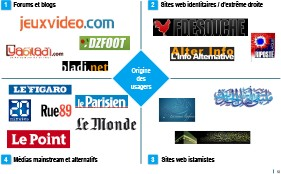
\includegraphics[width=\textwidth]{ImageIslamFrance/media/image10.jpeg}
\caption{L'islam sur YouTube}
\end{marginfigure}


YouTube est un élément clé du débat avec énormément de contenu publié et
relayé en rapport avec l'islam. En particulier, des dizaines de chaînes
sont tenues par des imams francophones, atteignant des dizaines de
milliers d'abonnements.

À cela s'ajoute d'innombrables vidéos sensation -- caméras cachées,
séquence émotion à la Mecque, exorcismes, extraits de débats, images
choc -- ainsi que des vidéos de musique et de récitations du Coran ; ces
dernières sont les plus performantes en termes de nombre de vues,
puisqu'elles sont utilisées comme musique de fond et jouées à
répétition.

L'offre idéologique islamique sur support vidéo Typologie et contenus


L'ensemble des discours auquel grand public a accès signale
l'\textbf{importance des}

\textbf{vidéos d'internet} dans la diffusion des idéologies islamistes.
Les vidéos les plus vues sur l'ensemble de la plateforme YouTube sont de
\textbf{cinq types} (par ordre décroissant en nombre de vues) :


\begin{itemize}
\item
  les \textbf{récitations coraniques :} vidéos très longues (60 minutes
  ou plus), de loin les plus vues (16 000 000). Leur large consommation
  est certainement due à un visionnage en « bruit de fond » ;
\item
  les \textbf{« vidéo buzz »} : brèves, liées à des sujets d'actualité :

  \begin{itemize}
  \item
    \textbf{laïcité :} des jeunes musulmanes empêchées d'entrer dans
    leur lycée ou dans des magasins à cause leur habillement (voile,
    gants, robes longues, etc.),
  \item
    \textbf{« people » :} des interviews de personnalités (Karim Achoui,
    rappeurs, etc.),
  \end{itemize}
\item
  \textbf{questions identitaires :} échos du conflit israélo-palestinien
  (LICRA, LDJ), rejet institutionnel et des médias \emph{« mainstream
  »}, perçus comme racistes. Ces vidéos sont souvent les plus politiques
  ;
\item
  les \textbf{vidéos « émotionnelles »} : des vidéos très courtes, au
  contenu religieux presque accessoire ; spiritualités émotives et
  émerveillement sentimental plutôt que la doctrine ; abondance de
  scènes «miraculeuses» ou dramatiques (enfants émus par l'appel à la
  prière, pleurs, etc.) ;
\item
  les \textbf{animations « spirituelles »} : des animations ou des
  vidéos de paysages avec un narrateur parlant de sujets spirituels, le
  plus souvent eschatologiques (signes avant-coureurs de l'apocalypse,
  etc.), très longues (5 à 6 heures)128 ; \textbf{les prêches et les «
  conférences »} : faites par les « Imams YouTube » (15 min- 1 h)129. Ce sont les discours les plus consommés.
\end{itemize}



Ces contenus diffusés sur YouTube n'offrent \textbf{pas une homogénéité
satisfaisante} pour les caractériser. Leurs points communs indiquent
cependant une \textbf{logique d'affirmation identitaire par le biais
d'islam(s)}. Cette construction identitaire est souvent explicitement
présentée comme étant en rupture avec certaines modernités qui
s'entremêlent :


\begin{itemize}
\item
  la consommation de masse ;
\item
  le rythme accéléré des communications qui détourne d'autrui et de ce
  qui est spirituel ;
\item
  un mode de vie jugé frivole, voire pécheur ;
\item
  des institutions perçues comme injustes ou hostiles.
\end{itemize}


L'immense majorité de ces productions proposent des contenus
difficilement compatibles avec les valeurs républicaines.


Des dynamiques de sens : construction d'un être au monde, d'interactions
du quotidien et du religieux


Les \textbf{vidéos de prêche} étonnent par la \textbf{trivialité de
leurs sujets.} Leur contenu n'est pas particulièrement heurtant pour le
grand public. Les questions traitées ont trait à des
\textbf{préoccupations courantes,} assez peu religieuses. Leur
\textbf{mise en scène} est très \textbf{simple}, parfois très
\textbf{théâtrale} (jeux de rôle caricaturaux), \textbf{emphatique}
(prêche depuis une tombe), et d'une \textbf{qualité technique très
limitée} (audio, vidéo et montage de faible qualité).

Les prêcheurs y répondent surtout à des questions au sujet de l'amour,
de conflits de couple, de \textbf{relations sexuelles,} de la
\textbf{réussite,} de l'\textbf{argent}, du rapport entre les
\textbf{parents et leurs fils,} de l'\textbf{amusement}. Les réponses
données sont assez semblables à celles que l'on attend de toute religion
sociale : les imams prônent la juste mesure, la bienveillance, la
générosité, la compréhension d'autrui, le dialogue, la tendresse, la
discipline.

Ce qui apparaît plus étonnant, c'est la \textbf{liturgie gestuelle et
verbale} orchestrant ces contenus triviaux. De l'ensemble des prêches
ressortent trois degrés de discours, accompagnés de dispositifs gestuels
:


\begin{itemize}
\item
  la plus grande partie de ces discours emprunte les \textbf{mots de la
  jeunesse} des banlieues. Très conscients du quotidien et des
  inquiétudes de leur auditoire, les orateurs veillent avec emphase à
  susciter l'adhésion à leur discours par des processus
  d'identification.
\item
  à ce discours du quotidien se mêle un \textbf{discours moral,
  théâtral, en français.}
\end{itemize}


Ce discours utilise un vocabulaire religieux, moral, au ton grave («
hélas »,
« miséricorde », « humilité ») ;


\begin{itemize}
\item
  le \textbf{troisième discours,} qui ponctue et \textbf{interrompt les
  deux précédents, est en arabe coranique.} Il s'agit de formules
  rituelles et de \textbf{récitations \emph{in extenso} de versets.}
\end{itemize}

Ces trois discours s'entremêlent. Il en ressort un discours qui établit
le religieux comme quotidien, et le quotidien comme religieux :


\begin{itemize}
\item
  la parole coranique vient ponctuer le langage de tous les jours, le
  sacralisant ;
\item
  le langage quotidien se trouve empreint de religiosité dans ses
  signifiés les plus triviaux.
\end{itemize}


La grande force de ce discours découle de cette mise en scène du sens,
qui lui confère une autorité absolue. Tout est religieux, la religion
est partout.


Promesse véhiculée


Cette élaboration discursive explique l'attrait de cette sorte de prêche
salafiste. \textbf{La promesse} téléologique de ces discours
\textbf{n'est pas historiquement révolutionnaire.} Comme tous les
millénarismes, \textbf{elle affirme la prompte arrivée de la fin des
temps,} et la justice qui y sera rendue.

L'appel qui y est fait, est de mener une vie qui plaise à Allah, afin de
garantir son salut. Cette vie est présentée comme difficile en raison
\textbf{du déluge de péchés} modernes. L'enfer guette tant qu'y échapper
est déjà presque un paradis. \textbf{La promesse est celle d'une justice
implacable.}

Il convient pourtant de signaler que cette justice est double : elle
s'exerce dans l'au-delà, dans l'éventualité du jugement dernier, mais
aussi ici-bas.

De nombreuses histoires édifiantes promettent que le péché commis
entraînera un châtiment dès la vie terrestre du pécheur ; se mêlent
ainsi à nouveau le quotidien et le transcendant, dans un être au monde
construit sur cette idée : \textbf{le trivial compte autant que le
religieux, le religieux est trivial, gestuel.} Le salut de l'âme se joue
chaque jour, chaque jour peut le mettre en péril.

En ce sens, la vie proposée est presque sans promesse : elle se promet
elle- même. Vivre comme le prophète et les \emph{salaf as-salih} est
déjà le paradis.

La réalité de l'islam français, avant d'être institutionnelle, est
d'abord locale et quotidienne. C'est un islam parcellaire, fragmenté et
éclaté, mais en voie d'intégration et de structuration au niveau local
qui se dessine. L'arrivée du
salafisme et sa visibilité attestent, paradoxalement, de la relative
bonne intégration de l'islam dans le paysage national. Parce qu'il se
fond dans le quotidien, l'islam des collectivités est difficile à
appréhender : il offre peu de de traits saillants à analyser et s'avère
être, par conséquent, un objet peu étudié ; seuls les mouvements
radicaux et minoritaires sont visibles. L'émergence rapide du salafisme
montre également, ainsi que le notait déjà en 2005 Samir Amghar, que
\emph{« la France est devenue un maillon de la globalisation du
religieux musulman, et constitue une plaque tournante pour de nombreux
flux transnationaux islamiques. Dans un tel contexte, comment concevoir
le contrôle de l'État, qu'il soit français ou qu'il s'agisse de l'État
d'origine ? La transnationalisation provoque une transformation des
relations entre l'islam et l'État, en de nouvelles formes d'autonomie et
de concurrence. La transnationalisation et la déterritorialisation des
mouvements islamiques donnent le primat aux leaders religieux et aux
chefs charismatiques, comme nous l'avons vu avec les théologiens
salafistes}\emph{. »}

Ce mouvement de transnationalisation et de déterritorialisation s'est
considérablement renforcé avec la démocratisation de l'accès à internet
et l'apparition des réseaux sociaux. Cette évolution de l'islam français
rend ainsi d'autant plus difficile, et d'autant plus urgent, le travail
de structuration de l'islam en France à la fois par les musulmans de
France et par la puissance publique.

130 Samir Amghar, Acteurs internationaux.


\subsubsection{Pistes de recommandation}


L'analyse du paysage de l'islam français permet d'éclairer la faiblesse
organisationnelle de l'islam en France. En partie soumis aux influences
étrangères, il peine à se structurer et à s'organiser. Les musulmans de
France, parce qu'ils forment une

« communauté introuvable », parce qu'ils présentent une grande diversité
à la fois ethnique et sociodémographique, ne parviennent pas à se doter
des structures nécessaires pour une gestion à la fois transparente,
structurée et régulée de l'islam français.

Les fondamentalistes ont pris une avance considérable dans plusieurs
domaines, mais, d'abord et avant tout, dans la diffusion de leur
idéologie. Dès lors, le combat doit être idéologique et culturel. Il
faut utiliser tous les moyens en notre possession pour soutenir les
musulmans dans le travail nécessaire qu'ils doivent mener
d'interprétation des textes et de diffusion des connaissances.
\textbf{La connaissance et la culture sont les enjeux premiers.}

\textbf{Le deuxième enjeu est le financement et l'organisation.} L'islam
de France est sous-financé, mal organisé et laisse place à des
offensives de groupes militants qui n'ont pas besoin de beaucoup de
moyens pour s'imposer, dans les mosquées et sur internet. Il faut donc
financer et organiser de façon transparente l'islam de France en
inventant, enfin, les moyens de s'affranchir des tutelles étrangères

Enfin, l'État doit comprendre que les mieux à même de gérer l'islam en
France, ce sont les Français, et non les États d'origine ni un CFCM dans
lequel les musulmans ne se reconnaissent pas. Il faut donc leur
permettre d'engager ces changements.




\hypertarget{propositions}{%
\paragraph{propositions}\label{propositions}}

 
\subparagraph{Réussir la création de la Fondation pour l'islam de
France, l'association musulmane pour un islam de France : deux
institutions
majeures} 

L'islam en France est confronté à un double défi : sortir enfin de la
tutelle des États étrangers et centraliser son organisation, avec
l'intérêt général des Français de confession musulmane comme principe
directeur.

L'islam de France doit devenir français. Il ne l'est pas aujourd'hui.
Les personnes qui le gèrent et celles qui représentent les musulmans
français sont encore étroitement liées aux États d'origine. Elles ont
importé les tensions qui existent entre certains États du Maghreb, ne
connaissent pas bien les jeunes Français avec qui elles sont pourtant
censées travailler et ne maîtrisent pas les outils de communication de
la jeunesse française.

Pourtant, trois musulmans sur quatre sont désormais des Français (dont
50 \% de naissance). Une nouvelle génération de musulmans français a
grandi en France et dispose d'un haut niveau de formation. Pour que
l'islam français puisse se doter d'une ligne théologique compatible avec
la société française et afin qu'il puisse rompre avec les discours
diffusés par les États émetteurs d'idéologies rigoristes, il faut créer
des instances capables de produire et de diffuser des idées et des
valeurs françaises.

Extrêmement fragmenté et divisé entre les États d'origines, les
mouvements transnationaux et les acteurs locaux, l'islam français doit
faire sa mue : il faut centraliser sa gestion afin de la rendre plus lisible et plus
efficiente. Cette maturation de l'islam français requiert aussi une
centralisation des moyens, un accroissement des capacités financières,
un effort de transparence et un contrôle accru avec un seul objectif :
l'intérêt général des musulmans de France et leur adhésion au pacte
républicain.

En août 2016, le ministre de l'Intérieur a annoncé la création d'une
Fondation pour l'Islam de France, dont Jean-Pierre Chevènement,
présidera le volet culturel131. Ses principales missions seront la
formation des imams et la production de connaissances sur l'islam.

Il faudra lui accoler une association cultuelle régie par la loi de 1905
pour pouvoir financer ce qui est du strict ressort cultuel (construction
des lieux de culte, salariat des imams, formation théologique). Le
Conseil d'État a contesté le fait qu'une fondation d'utilité publique
puisse contribuer au financement du culte On pourrait appeler cette
association « l'association musulmane pour un islam de France (AMIF) ».
Pour y parvenir, il faut proposer une nouvelle gouvernance et une
nouvelle génération pour les deux organisations.

\textbf{Trois propositions pour la gouvernance et l'organisation de ces
deux institutions.}


Gouvernance proposée pour ces deux institutions


Ainsi, pour leur premier mandat, au conseil d'administration de ces
organisations, une majorité de ces Français de confession musulmane
devront être cooptés par l'État. Pourquoi par l'État ? Parce qu'il
s'agit d'une fondation reconnue d'utilité publique, et parce que l'État
aura conféré à l'association le monopole de la délivrance de carte de
certification, permettant ainsi le monopole religieux. Mais aussi parce
que l'État devra assumer la nécessité de renouveler à la fois les
générations et l'organisation. Cette nouvelle génération siègera avec, à
ses côtés, des représentants du CFCM qui devront être
\textbf{minoritaires} dans l'organisation.

Ces nouveaux membres, capables de fédérer la communauté musulmane et de
lever des fonds pour le financement du culte musulman, auront une double
mission : centraliser les flux financiers liés à l'exercice de la
religion et organiser

131 On ne peut que s'étonner qu'une personnalité non musulmane préside
la Fondation de l'islam de France. Cependant, Jean-Pierre Chevènement
pourra être le préfigurateur de la Fondation, en lien avec le futur
président de l'association cultuelle, avant de passer la main dans un
délai aussi bref que possible à une personnalité musulmane.



l'emploi efficace et transparent de ces ressources. Le Conseil
d'administration des deux organisations ainsi nommé aura également pour
mission de mettre au point le dispositif qui permettra de renouveler sa
composition au terme de ce premier mandat, \emph{via} un système
représentatif


Une nouvelle équipe


La réactivation de la FIF et la création de l'AMIF devront s'accompagner
d'un profond renouvellement des représentants et des acteurs de l'islam
français. Il est temps de faire émerger \textbf{une nouvelle génération
de musulmans, qui ont grandi et ont été socialisés en France et de
profiter de la volonté qu'ils ont manifestée.} Il revient à la puissance
publique d'accompagner l'émergence de cette nouvelle génération de
musulmans français, en la nommant au conseil d'administration et à la
direction générale de la Fondation ; aux côtés de membres du CFCM, qui
ne devront composer que moins de la moitié du Conseil d'administration
de la FIF et de l'AMIF. Cette nouvelle génération devra également
investir les conseils régionaux de la Fondation, qui seront composés de
personnalités désignées, pour ce premier mandat, par les autorités
publiques et des membres du CFCM.


Une mission principale : centraliser les flux financiers


\textbf{La Fondation pour l'islam de France (FIF) et l'AMIF,} doivent
devenir la clef de voûte de la nouvelle gestion de l'islam français.
Forte de l'ensemble des financements liés à l'exercice religieux, l'AMIF
financera les lieux de culte, formera et salariera les imams et
financera le travail théologique. La Fondation limitera le champ de son
action au domaine culturel. Ces revenus financiers procèderaient de
quatre sources différentes :


\begin{itemize}
\item
  \textbf{le monopole des cartes de sacrificateurs musulmans.}
  Actuellement, trois mosquées (liées pour deux d'entre elles
  explicitement à des pays étrangers, l'Algérie pour la mosquée de Paris
  et le Maroc pour la mosquée d'Évry) bénéficient d'un agrément donné
  par le ministère de l'Agriculture sur proposition du ministère de
  l'Intérieur pour délivrer des cartes de sacrificateurs religieux. Ces
  sacrificateurs rendent un service qui est rémunéré par les abattoirs
  dont le produit sert au financement des mosquées qui en bénéficient et
  des associations qui leur sont proches.
\end{itemize}


L'AMIF (l'association cultuelle) devra être demain la seule titulaire de
l'agrément afin de pouvoir centraliser les flux financiers liés à
l'abattage \emph{halal} (quitte à passer par une structure juridique
\emph{ad hoc} si besoin est). L'AMIF s'engagera à reprendre les
 sacrificateurs qui travaillent actuellement pour les mosquées agréées et
proposera aux mosquées une compensation sur une base transparente, pour
autant que le produit actuel du service des sacrificateurs serve la
communauté musulmane.

L'AMIF (association loi de 1905), seule titulaire de l'agrément, pourra
ensuite faire évoluer les tarifs des sacrificateurs, dans l'intérêt des
fidèles, après avoir évalué les besoins de financement du culte musulman
en France et les différentes sources de recettes.

Il y aura bien sûr des difficultés (pourquoi augmenter le prix des
services ? pourquoi retirer l'agrément à des mosquées qui n'ont pas
démérité ? pourquoi prélever plus d'argent sur des gens disposant
souvent de peu de ressources ?) mais, avec le service de certification,
la redevance pour l'abattage \emph{halal} est une source majeure de
financement qu'il faut utiliser jusqu'au bout ;


\begin{itemize}
\item
  \textbf{une offre de certification \emph{halal} sur toute la chaine de
  valeurs.} Il est impossible de créer une taxe halal, compte tenu du
  périmètre fluctuant de la définition du halal, du respect nécessaire
  de la liberté de commerce et de la concurrence, et du principe
  constitutionnel d'égalité des citoyens devant l'impôt. Il est
  toutefois possible de doter l'AMIF d'une mission de certification du
  \emph{halal} sur l'ensemble de la chaîne de valeur, qui viendrait
  concurrencer les acteurs déjà présents sur ce marché. Conformément au
  droit de la concurrence et au respect de la liberté d'entreprendre,
  l'AMIF n'aurait pas le monopole de la certification du \emph{halal},
  mais aurait à charge de savoir déployer un vrai service de
  certification en se fondant sur sa légitimité nationale, sur la
  transparence de ses coûts et surtout sur l'utilisation de ses
  bénéfices au service de la collectivité ;
\item
  l\textbf{e recueil des dons versés par des pays ou des personnalités
  étrangères.} Il règne actuellement une véritable opacité autour des
  dons versés par les pays et les personnalités étrangères aux
  associations musulmanes. Il est nécessaire d'introduire de la
  transparence, et surtout de rompre l'affiliation de certaines
  associations avec les pays d'origine. C'est pourquoi ces flux
  financiers devront être progressivement réorientés et transiter
  obligatoirement par la FIF, afin de permettre une centralisation -- en
  toute transparence -- du financement étranger de l'islam français ;
\item
  \textbf{le recueil d'une redevance sur le pèlerinage,} en lien avec
  les agences de voyage qui l'organisent ;
\end{itemize}





\begin{itemize}
\item
  \textbf{le recueil de dons (zakat) venus des fidèles français.} La
  zakat représente, tout comme les financements étrangers, une
  importante source de financement de l'islam français. Or, ce mode de
  financement est totalement opaque, fragmenté et parcellaire. Il est
  nécessaire d'y introduire de la transparence, et surtout de mutualiser
  au sein de la Fondation les ressources provenant des fidèles : cette
  centralisation du financement des fidèles permettra à l'islam français
  de se structurer et de se professionnaliser ; et par là même de mieux
  s'intégrer dans la République. On pourra imaginer d'utiliser des
  moyens modernes de dons, comme par exemple des applications sur
  smartphones.
\end{itemize}


L'AMIF sera des deux organisations celle qui aura vocation à recueillir
le plus d'argent, les besoins de financement étant essentiellement liés
à l'exercice du culte. La Fondation pourra recevoir des dons de
personnes physiques, sachant que son action sera strictement limitée au
domaine culturel, conformément à la loi de 1905 et à la séparation de
l'Église et de l'État.


L'usage des fonds


Les fonds recueillis et centralisés par la FIF auront plusieurs emplois
:


\begin{itemize}
\item
  \textbf{financer la construction de lieux de culte :} toute
  construction de mosquée devra être préalablement visée par la FIF et
  son plan de financement certifié par son équipe dirigeante ;
\item
  \textbf{salarier les imams :} tout imam ayant passé avec succès le «
  Test de l'islam français » (détail ci-après) administré par l'AMIF
  pourra être salarié par cette association. La centralisation des
  ressources et la garantie d'un discours théologique compatible avec
  les valeurs et les principes de la République permettront l'émergence
  d'un islam français ;
\item
  \textbf{former les imams :} en plus de la reconnaissance -- ou non --
  des imams déjà en fonction, la Fondation aura pour mission de former
  une nouvelle génération d'imams. La centralité de l'AMIF, clef de
  voûte de l'islam français, permettra ainsi de mettre fin à la
  délégation de la formation des imams à des pays étrangers ou à des
  instituts privés. L'objectif est de garantir que les tous les imams en
  France soient français -- ou maîtrisent le français -- et aient suivi
  la formation d'une institution reconnue par la République et
  compatible avec ses idéaux ;
 
\item
  \textbf{rémunérer l'équipe de l'AMIF, de la Fondation et des
  sacrificateurs :} la FIF, en plus de la rémunération des personnes
  chargées du fonctionnement administratif de l'islam français, devra
  salarier les sacrificateurs \emph{halal} auxquels elle aura délivré
  des accréditations ;
\item
  \textbf{engager un travail idéologique :} à terme, une fois la
  centralisation des flux financiers durablement assurée et les
  institutions nécessaires à l'émergence d'un islam français solidement
  implantées, la FIF aura pour mission d'engager une véritable bataille
  culturelle, sur le web et sur le terrain, afin de réduire l'emprise
  des discours islamistes, salafistes et djihadistes sur les musulmans
  de France.
\end{itemize}


La réactivation de la FIF, la création de l'AMIF, la centralisation des
flux financiers, un usage responsable des fonds et l'arrivée d'une
nouvelle génération de musulmans français doivent permettre l'émergence
d'un islam français, mais aussi de mettre un terme à sa fragmentation et
à sa gestion externalisée, afin d'être en mesure de répondre aux défis
auxquels il fait face aujourd'hui.
 
\subparagraph{Un grand imam de France pour exprimer une doctrine
musulmane compatible avec les valeurs
républicaines} 


Afin de désigner un interlocuteur musulman légitime et représentatif aux
pouvoirs publics, nous recommandons l'élection d'un Grand Imam de
France. Celui-ci devra être de nationalité française, diplômé de
théologie, imam d'une mosquée et avoir recueilli le parrainage de
présidents d'associations cultuelles. Il sera élu par le Conseil
d'administration de l'AMIF et, éventuellement, un collège élargi avec
des personnalités qualifiées. Il portera un discours et une ligne
idéologique qui puisera au plus profond des valeurs spirituelles de
l'islam tout en étant en adéquation avec la société française du XXIe
siècle. Il sera le représentant spirituel de l'islam français
-- aux côtés des présidents du CFCM et de l'AMIF --et aura pour mission
d'intervenir, à l'instar du Grand Rabbin de France, dans les médias --
ou auprès d'institutions désireuses de recueillir un éclairage
théologique sur certaines questions -- afin de mieux faire connaître
l'islam. Il devra également conduire le travail intellectuel et
théologique destiné à poser les jalons d'un islam français. Pour cela,
il devra interagir avec tous les imams de France. Il pourra, en accord
avec l'AMIF, les révoquer en 
cas de discours déviant ou de prises de positions contraires au
vivre-ensemble. Il s'appuiera pour cela sur des représentants religieux
régionaux.

Si le Grand Imam de France sera chargé de représenter les ministres du
culte musulman, les responsables de l'AMIF auront également pour mission
d'être le visage des musulmans français et de parler au nom de cette
majorité silencieuse, bien intégrée dans la République française et
première victime de l'islamisme et du radicalisme religieux.

 \subparagraph{Élargissement du concordat alsaco-mosellan à
l'islam} 
\textbf{Un régime particulier conforté par le législateur, le Conseil
d'État et le Conseil constitutionnel}

L'Alsace-Moselle jouit d'un régime cultuel différent de celui du reste
de la métropole : la loi de 1905 ne s'y applique pas. Cette
particularité s'explique par la situation de ces départements qui
étaient sous occupation allemande en 1905. Conformément aux dispositions
qui courraient avant l'application de la loi de 1905, les quatre cultes
« reconnus » (le culte catholique, les cultes protestants luthérien et
réformé et le culte judaïque) sont pris en charge par la puissance
publique, qui finance l'intégralité du culte, nomme et révoque les
ministres du culte, et assure pour chacun de ces cultes un enseignement
religieux (facultatif aujourd'hui) à l'école publique.

\textbf{Cette disposition dérogatoire au droit commun n'a pas été remise
en cause} et a été entérinée par la loi du 1er juin 1924132 et par un
avis du Conseil d'État en 1925133. Ce régime juridique applicable aux
cultes en Alsace-Moselle a été réaffirmé à plusieurs reprises depuis.
L'ordonnance du 15 septembre 1945, en maintenant en vigueur le droit
applicable le 16 juin 1940, confirme l'application du régime
concordataire en Alsace-Moselle. En 2001, dans sa décision
\emph{Syndicat national des enseignements du second degré,} le Conseil
d'État a également rappelé que \underline{les principes fondamentaux
reconnus par les lois de la République, au nombre}
desquels figure le principe de laïcité dans les préambules des
constitutions des 27 octobre 1946 et 4 octobre 1958 \emph{« n'a pas eu
pour effet d'abroger implicitement les dispositions de ladite loi ».}

Dernièrement, en 2013, c'est le Conseil constitutionnel qui a confirmé
la constitutionnalité de cette disposition particulière. Ainsi, à
l'occasion de la question prioritaire de constitutionnalité (QPC)
\emph{Association pour la promotion et l'expansion de la laïcité,}
\textbf{le juge constitutionnel a affirmé à son tour que le régime
concordataire qui prévaut encore en Alsace-Moselle n'est pas entaché
d'inconstitutionnalité}\sn{ CC, Décision n'° 2012-297 QPC du 21 février 2013. Voir notamment le sixième considérant : « \emph{Considérant, toutefois, qu'il ressort tant
des travaux préparatoires du projet de la Constitution du 27 octobre
1946 relatifs à son article 1er que de ceux du projet de la Constitution
du 4 octobre 1958 qui a repris la même disposition, qu'en proclamant que
la France est une ``République. . . laïque'', la Constitution n'a pas
pour autant entendu remettre en cause les dispositions législatives ou
règlementaires particulières applicables dans plusieurs parties du
territoire de la République lors de l'entrée en vigueur de la
Constitution et relatives à l'organisation de certains cultes et,
notamment, à la rémunération de ministres du culte ; »} (nous
soulignons).}\textbf{.}


La situation de l'islam dans le régime concordataire


Aujourd'hui, \textbf{l'islam n'est pas intégré au régime concordataire}
alsacien et mosellan. C'est \textbf{un culte « non-reconnu ».} Par
conséquent, le financement du culte musulman -- et plus largement celui
des nouveaux cultes -- n'est pas aligné sur le régime dont bénéficient
les quatre cultes reconnus. En revanche, \textbf{les associations -- en
vertu du droit local -- peuvent recevoir des soutiens financiers publics
et les collectivités peuvent participer au financement d'une partie des
cultes non-reconnus} (en respectant cependant un certain nombre de
règles). C'est ainsi que la mairie de Strasbourg, le département du
Bas-Rhin et la région Alsace ont participé au financement de la
construction de la Grande Mosquée de Strasbourg à hauteur de 1,6 million
d'euros, soit un quart du coût total de l'édifice. Toutefois, le régime
concordataire empêche les pouvoirs publics de prendre en charge la
totalité du culte et de pouvoir nommer et salarier des imams. Pour ainsi
dire, \textbf{si la puissance publique peut en partie financer le culte
musulman en Alsace-Moselle, elle ne peut en revanche pas en réguler le
fonctionnement.}

\textbf{Parce que le régime concordataire est protégé aussi bien par le
législateur que par le Conseil d'État ou le Conseil Constitutionnel,
certains ont envisagé d'y intégrer l'islam, afin de permettre aux
pouvoirs publics de participer plus avant au fonctionnement de ce
culte.} Cette idée n'est pas nouvelle. Déjà, en 1997, alors qu'il était
au ministère de l'Intérieur, Jean-Pierre Chevènement songeait à utiliser
ce régime dérogatoire pour en faire un laboratoire de l'islam français
et créer une université de théologie islamique à Strasbourg.

C'est également l'idée du député François Grosdidier lorsqu'il dépose,
en 2006, une proposition de loi visant à intégrer le culte musulman dans
le régime concordataire d'Alsace et de Moselle afin de mettre fin à une
situation inégalitaire. Selon lui, étant donné \textbf{que les nouveaux
cultes, au premier rang desquels l'islam, se trouvent dans une situation
défavorable au regard de celle des cultes reconnus dans les trois
départements de l'Est,} il se prononçait en faveur \emph{\textbf{« d'une
actualisation de la loi concordataire »}} en direction de l'islam.
Reprenant l'idée développée par Jean- Pierre Chevènement, il se
prononçait également en faveur de la création d'une chaire de théologie
islamique à l'université de Strasbourg, dont les travaux pourraient
contribuer à l'émergence d'un islam français.

Au-delà des raisons politiques qui ont conduit au non-examen de ce texte
et des raisons juridiques -- du risque d'inconstitutionnalité de cette
proposition de loi --, \textbf{le Conseil Constitutionnel a clos jusqu'à
nouvel ordre le débat public autour de cette question en 2011.} En
effet, dans sa décision \emph{Société SOMODIA,} relative à
l'actualisation du régime concordataire en Alsace et Moselle, il a
rappelé que si le législateur ou le pouvoir réglementaire pouvaient
maintenir, atténuer ou même supprimer les dispositions du droit local,
\textbf{ils ne pouvaient pas en revanche, en élargir le champ
d'application.} Si la dérogation au droit commun demeure l'exception,
son approfondissement n'est pas souhaitable, car il risquerait
d'accroître l'inégalité des citoyens devant la loi. \textbf{Le juge
constitutionnel a signifié ainsi que les cultes nouvellement installés
sur le territoire français ne peuvent, en Alsace- Moselle, bénéficier du
même régime juridique que les cultes reconnus}\sn{135 Décision n°2011-157 QPC du 5 août 2011. Voir notamment le quatrième
considérant : Considérant qu'ainsi, la législation républicaine
antérieure à l'entrée en vigueur de la Constitution de 1946 a consacré
le principe selon lequel, tant qu'elles n'ont pas été remplacées par les
dispositions de droit commun ou harmonisées avec elles, des dispositions
législatives et réglementaires particulières aux départements du
Bas-Rhin, du Haut-Rhin et de la Moselle peuvent demeurer en vigueur ;
qu'à défaut de leur abrogation ou de leur harmonisation avec le droit
commun, ces dispositions particulières ne peuvent être aménagées que
dans la mesure où les différences de traitement qui en résultent ne sont
pas accrues et que leur champ d'application n'est pas élargi ; que telle
est la portée du principe fondamental reconnu par les lois de la
République en matière de dispositions particulières applicables dans les
trois départements dont il s'agit ; que ce principe doit aussi être
concilié avec les autres exigences constitutionnelles » (nous
soulignons)}\textbf{.} Ainsi, en
2011, le Conseil Constitutionnel a fermé la voie à toute tentative de
faire de l'Alsace-Moselle un théâtre d'expérimentation et le lieu
d'émergence d'un islam
\emph{« made in France ».}

Nécessité et modalités d'intégration de l'islam au régime concordataire

Nécessité

Il est, aujourd'hui plus que jamais, nécessaire \textbf{d'intégrer
l'islam au régime concordataire.} Il ne s'agit pas de faciliter le
financement du culte musulman, mais de créer un écosystème politique et
juridique qui permette aux instances représentatives des musulmans de
France et à la puissance publique de \textbf{faire émerger un islam
français,} dont les discours et la pratique soient en adéquation avec
les évolutions de notre société.

L'actualisation du régime concordataire doit offrir la possibilité de
\textbf{créer une chaire de théologie musulmane} à l'Université de
Strasbourg, dont la mission consisterait à produire de la connaissance
sur l'islam à destination des Français, ainsi qu'à élaborer un discours
théologique compatible avec les attentes de la société et les exigences
de la République.

L'Alsace-Moselle pourrait également accueillir \textbf{une école de
formation des imams.} En créant un diplôme français de théologie
islamique, l'État répondrait à une forte attente des musulmans de
France. Surtout il se donnerait les moyens, sur le temps long, de
diffuser auprès des fidèles musulmans un discours adapté aux valeurs de
notre société.


Modalités


\emph{Revenir sur la jurisprudence Société Somodia}

L'intégration de l'islam au régime concordataire implique, tout d'abord,
de \textbf{revenir sur la jurisprudence du Conseil constitutionnel.} En
effet, si en 2011 le juge constitutionnel avec la décision sur le QPC
\emph{Société Somodia} a sécurisé le droit local des cultes
(sécurisation qui sera confirmée en 2013 avec la QPC \emph{Association
pour la promotion et l'expansion de la laïcité}), il a en revanche
\textbf{verrouillé toute possibilité d'actualisation du droit
concordataire :} l'intégration de nouveaux cultes dans le régime
concordataire constituerait un approfondissement et un élargissement
trop important d'un droit local par nature dérogatoire.

Cette actualisation du régime concordataire implique donc de recourir à
une loi, \textbf{afin que celle-ci soit déférée devant le Conseil
constitutionnel,} et non d'emprunter la voie réglementaire au risque de
voir le Conseil d'État censurer le texte en raison de
son inconstitutionnalité manifeste. Il faut ensuite que \textbf{les
juges constitutionnels}
-- au regard des circonstances présentes et des dispositions du projet
de loi -- \textbf{procèdent à un revirement de jurisprudence.} Cette
évolution jurisprudentielle pourrait s'opérer autour de la nécessité de
réduire l'inégalité de situation à laquelle sont confrontés les fidèles
des cultes reconnus et ceux des cultes non-reconnus et qui porte
potentiellement atteinte à la liberté de culte -- et non autour de
l'application uniforme du droit sur l'ensemble du territoire ou de
l'objectif de réduction des dispositions particulières dérogatoire au
droit commun, qui structurent la décision \emph{Société Somodia}. Le
nouveau contexte politique et social, né des attentats de 2015 et de
2016, pourrait justifier cette évolution.

\textbf{Cette évolution jurisprudentielle serait loin d'être anodine,
car le Conseil constitutionnel n'est jamais revenu sur une décision
prise dans le cadre d'une QPC.} Assurément, ce revirement ferait
jurisprudence et risquerait fort d'agiter la doctrine juridique. Aussi,
au-delà des considérations politiques que soulève l'intégration de
l'islam au régime concordataire, il convient de \textbf{prendre en
compte l'ensemble des obstacles juridiques que rencontrera cette
proposition.}

\textbf{Comment « reconnaître » le culte musulman ?}

\textbf{Le terme de « reconnaissance » est impropre,} ainsi que le
rappelle fort à propos le rapport rédigé par Jean-Pierre Machelonde 2006
:
\begin{quote}
    \emph{« aucune loi n'a jamais reconnu explicitement les cultes
catholique, protestant et israélite. En revanche, ceux-ci ont engagé au
cours du XIXe siècle des négociations avec l'État débouchant, après une
période plus ou moins longue (50 ans pour le culte israélite) sur ce qui
peut être qualifié « d'arrangements statutaires ». Ces statuts
particuliers sont donc propres à chaque culte. {[}\ldots{]} Les cultes
statutaires ne constituent donc pas un ensemble homogène, et l'islam,
avec ses caractéristiques particulières, peut sans nul doute y trouver
sa place}\emph{. »}
\end{quote}

\textbf{Ce rapport publié en 2006, soit avant la QPC \emph{Société
Somodia,} propose de procéder à la « reconnaissance » du culte musulman}
en recourant à des dispositions règlementaires (recrutement des
ministres du culte musulman, création d'établissements du culte
musulman, etc.) afin d'amorcer un effet « cliquet » et de faciliter
l'introduction d'autres dispositions, qui relèvent de matières
législatives. Compte tenu de l'état actuel du droit et de la situation
jurisprudentielle, l'introduction
du culte musulman dans le régime concordataire ne saurait s'effectuer de
manière

\emph{« pragmatique et progressive ».} Il faut d'emblée se situer au
niveau législatif afin que le texte soit visé par le Conseil
constitutionnel.

Par ailleurs, au regard de l'exigence de neutralité de l'État à l'égard
des cultes et de son corollaire -- l'égalité de traitement des
différents cultes qui prévalent dans les régimes juridiques dérogatoires
au droit commun des cultes --, \textbf{il importe de veiller à ce que
le texte législatif visant à élargir à l'islam le régime concordataire
ne soit pas exclusif au seul culte musulman.} Par conséquent, s'il faut
procéder à l'actualisation du concordat alsacien-mosellan, il convient
de \textbf{l'ouvrir à l'ensemble des nouveaux cultes qui le
souhaiteraient} -- soit, compte tenu des pratiques cultuelles locales,
le culte orthodoxe, le culte protestant évangéliste et le culte
musulman, principalement.

C'est pourquoi, conformément à l'article 34 de la Constitution, deux
pistes non exclusives paraissent envisageables :


\begin{enumerate}
\def\labelenumi{\alph{enumi}.}
\item
  compte tenu du fait que les textes relatifs au droit local
  d'enseignement religieux ne se réfèrent pas à la notion de « cultes
  reconnus », \textbf{un projet ou une proposition de loi relatifs à la
  création de postes de professeurs non contractuels d'enseignement des
  religions musulmane,} orthodoxe et évangéliste permettraient au
  Conseil constitutionnel d'examiner le texte et de se prononcer en
  faveur d'un éventuel revirement de jurisprudence ;
\item
  
  en collaboration avec le CRCM, qui constitue l'instance représentative
  locale des musulmans, et \textbf{dans le cadre d'une loi de finance,
  un amendement relatif à la rémunération des ministres des cultes
  musulman,} orthodoxe et évangéliste, doit offrir la possibilité au
  Conseil constitutionnel -- dans le cadre de l'examen de
  constitutionnalité du PLF -- d'effectuer un revirement de
  jurisprudence sur le régime applicable au culte en Alsace-Moselle.
  
\end{enumerate}


Il est évident que ces deux voies ne constituent qu'\textbf{une première
étape dans la création d'un statut du culte musulman} et que leur
ambition est plus large que la structuration du seul culte musulman. Il
s'agit toutefois d'un passage obligé avant la création d'un véritable
écosystème politique, juridique et intellectuel propice à l'émergence
d'un islam français. Sans cette étape législative déterminante, il sera
{impossible de mettre en place ultérieurement une formation
diplômante en théologie}
desdits professeurs non contractuels, ni de créer une chaire de
théologie islamique au sein de l'Université de Strasbourg.


Risques


Quels sont les risques que présente l'élargissement du régime
concordataire à de nouveaux cultes ? Si \emph{a priori} une telle mesure
ne soulève pas de véritable risque financier (voir après) et si le
risque juridique d'inconstitutionnalité est levé, les principaux risques
qui pèsent sur cette mesure sont politiques.


\begin{enumerate}
\def\labelenumi{\alph{enumi}.}
\item
  Cette mesure suscitera sans aucun doute \textbf{l'opposition des
  partisans de l'abolition du régime concordataire, qui ne sont pas
  favorables à une prise en charge des cultes par la puissance
  publique.} Il est indéniable que c'est une opposition à prendre en
  compte, et qui sera particulièrement virulente à l'occasion de
  l'examen des textes de lois.
\item
  
  \textbf{L'opposition des cultes « reconnus » dans le cadre du régime
  concordataire doit également être intégrée.} Ils exprimeront une
  double crainte. Ils risquent de voir dans cette mesure un risque de
  péréquation budgétaire défavorable à leur égard, d'une part ; ils ne
  manqueront pas d'agiter la menace d'un risque de rupture du régime
  concordataire, d'autre part. Son extension signifierait alors son
  abrogation. Toutefois, la décision de 2013 du Conseil Constitutionnel
  constitue une véritable sécurisation, au plus haut niveau
  juridictionnel, de ce dispositif politique et juridique.
  
\item
  
  Enfin, il est très probable qu'\textbf{une partie des musulmans sera
  opposée à la gestion du culte par la puissance publique.} L'offre
  consulaire est relativement importante en Alsace-Moselle, où les
  musulmans sont principalement d'origines marocaine et turque : la
  création d'un corps de fonctionnaires français en charge du culte
  musulman et l'émergence consécutive d'une offre d'islam français
  entraîneront des perturbations locales et diplomatiques qu'il convient
  d'anticiper afin de les atténuer. En outre, certains responsables
  d'associations cultuelles locales seront réticents face à une telle
  implication de l'État dans les affaires cultuelles, \textbf{car la
  prise en charge publique des cultes implique en contrepartie un
  important droit de regard et de contrôle de leur fonctionnement.}
  
\end{enumerate}

Coût de l'élargissement du régime concordataire à l'islam


\textbf{Le coût d'une telle mesure s'établirait entre 5,5 et 6 millions
d'euros,} et se répartirait comme suit :


\begin{itemize}
\item
  au regard de la population musulmane et du nombre de mosquées en
  Alsace- Moselle, il faudrait procéder à la rémunération d'\textbf{une
  soixantaine de fonctionnaires du culte,} qui pourront assurer aussi
  bien la formation religieuse scolaire que le ministère du culte. Avec
  un salaire mensuel compris entre 1 800 et 2 000 e, \textbf{nous
  estimons que la création d'un corps de fonctionnaires du culte
  musulman s'élèverait à 2,5 millions d'euros par an environ ;}
\item
  la \textbf{création d'une chaire de théologie islamique au sein de
  l'Université de Strasbourg,} qui compterait dans un premier temps une
  petite dizaine de professeurs, est estimée \textbf{entre 1 million et
  1,5 million d'euros par an ;}
\item
  enfin, \textbf{la prise en charge de la construction des édifices
  cultuels par la puissance publique, ainsi que leur entretien,
  coûterait environ 2 millions d'euros annuels,} en intégrant à ce
  calcul la construction de nouvelles mosquées.
\end{itemize}


L'ensemble de ces dépenses suppose une pleine et entière intégration de
l'islam au régime concordataire. \textbf{L'accession de l'islam au
statut de « culte reconnu » sera le fruit d'une sédimentation de
mesures,} dont il est difficile d'évaluer le coût strate par strate. Il
est toutefois probable qu'\textbf{une telle évolution prendra plusieurs
années}

-- compte tenu à la fois du délai nécessaire à l'élaboration des
enseignements de religion musulmane et de celui requis pour la création
d'une chaire théologique. Aussi, le coût annuel de l'intégration de
l'islam au régime concordataire sera moindre durant les premières
années.


\subsection{L'enseignement de la théologie islamique en France et la formation des
imams}


L'analyse de l'offre et de la demande d'enseignement de l'islam à
l'université, depuis les années 1980 et 1990, fait apparaître
\textbf{deux dynamiques d'offre répondant à deux types de demandes.}


Une offre publique composite et incomplète


\textbf{Une dynamique de préconisation d'offre publique a émergé, sous
impulsion politique et universitaire, soutenue par les recommandations
de divers rapports publics :} création d'un enseignement religieux dans
les écoles en Alsace et en Moselle, préconisée par la Commission de
réflexion sur l'application du principe de laïcité dans la République
(Rapport Stasi, 2003), la Commission sur les relations des cultes avec
les pouvoirs publics (Rapport Machelon, 2006) et la Commission sur le
port du voile intégral sur le territoire national (Rapport Gérin, 2010).

Des universitaires (Mohamed Arkoun et Etienne Trocmé) ont inlassablement
tenté de sensibiliser les dirigeants politiques français et de formuler
une réponse à la demande d'enseignement religieux dans le cadre de la
loi de 1905.

Cette dynamique d'offre publique, mue par une volonté de création tantôt
d'une faculté de théologie musulmane à Strasbourg, tantôt d'un institut
islamique (Pierre Joxe et Alain Boyer en 1987), voire d'une École
nationale d'études islamiques fondée sur le modèle de l'École normale
supérieure (commission Stasi en 2003), pour former des enseignants à
l'enseignement du fait religieux et plus particulièrement l'enseignement
de l'islam et de la théologie islamique dans le supérieur.

\textbf{En 1997,} Jean-Pierre Chevènement relance l'idée d'un « institut
universitaire des hautes études de l'islam » ou des « études supérieures
islamiques » pour former des cadres musulmans au sein de l'Institut
national des langues et civilisations orientales (INALCO).

Entre 2005 et 2010, les facultés d'Aix-en-Provence, de Paris IV -- La
Sorbonne, puis de Paris 8 - Saint-Denis, ainsi que plusieurs
établissements publics, ont
tenté d'organiser des formations destinées aux futurs imams. La seule
initiative qui ait vu le jour est celle de l'Institut Catholique de
Paris, qui a créé, en 2008, un diplôme universitaire (DU) :
«Interculturalité, laïcité, religions ».

\textbf{En 2009,} le master d'islamologie de l'Université de Strasbourg
est ouvert. Cette formation offre un cadre général de formation d'imams
républicains.

\textbf{En 2016, une palette de treize offres publiques disparates et
éclatées de formations, d'enseignements et de diplômes existe.} Après
Paris, Lyon, Strasbourg, puis Montpellier, Aix et Bordeaux, sept nouveau
DU ont vu le jour en septembre 2015 à Sceaux, Paris 1, Lille, Toulouse,
Mayotte, Nantes et La Réunion.


Une offre privée de formation assez disparate


Il existe une dynamique d'offre privée, développée à l'initiative de
particuliers, d'associations ou de collectifs musulmans désirant
répondre à une demande de formation théologique des imams, de «
catéchèse musulmane » et d'exégèse du texte coranique.

Ainsi :


\begin{itemize}
\item
  en 1990, l'UOIF crée, à Saint-Léger de Fougeret, l'Institut européen
  des sciences humaines (IESH). Les frais de scolarité sont de 6 000
  euros par an ;
\item
  en 1993 est créée, sous l'impulsion financière saoudienne,
  l'Université islamique de France, à Mantes-la-Jolie ; elle est devenue
  en 1995 l'Institut d'études islamiques de Paris ;
\item
  en 1994, Dalil Boubakeur et Charles Pasqua sont à l'initiative de
  l'Institut Ghazali de formation des imams ;
\item
  en 1999 est créé l'Institut international des sciences islamiques
  (ISSI), qui propose une formation fondée sur le rite malékite ;
\item
  en 1999 l'International Institute of the Islamic Thought (IIIT),
  ouvert aux États- Unis en 1981, ouvre un établissement français :
  l'institut international de la pensée islamique à Saint-Ouen, en
  Seine-Saint-Denis ;
\item
  en 2001 est fondé l'Institut français des études et sciences
  islamiques (IFESI), à Boissy-Saint Léger, dans le Val-de-Marne ;
\item
  en octobre 2002, la Grande Mosquée de Paris relance son cursus de
  formation des imams, afin de former théologiquement des imams et des
  aumôniers femmes ;
\end{itemize}





\begin{itemize}
\item
  en 2006 est créé à Lille l'Institut Avicenne des Sciences humaines
  (IASH), qui a pour ambition de former les imams. L'Institut Avicenne
  réserve l'accès à son cursus aux seuls candidats justifiant de
  l'exercice de la fonction d'imam ou de responsable associatif depuis
  au moins six mois.
\end{itemize}

La formation des cadres religieux musulmans en Europe


Les modes de formation des cadres religieux musulmans en Europe
dépendent des statuts des cultes nationaux dans chaque pays.

\textbf{En Belgique,} le culte musulman est reconnu par l'État depuis
1974. L'Exécutif des musulmans de Belgique, équivalent du CFCM français,
a proposé en 2006 la création d'un statut des ministres du culte
musulman et la mise en place d'une formation à l'imamat de quatre à cinq
ans (théologie et formation civile et civique). Ce projet, demeuré
lettre morte, a été relancé en 2013.

En 2007, a été créée sur une initiative privée, une Faculté des sciences
islamiques de Bruxelles. Celle-ci a en 2008 signé une convention avec
l'université islamique européenne de Rotterdam, proche du mouvement turc
Nursi, et dispose d'un département en charge de la formation des imams.
Les diplômes qu'elle délivre ne sont pas reconnus par l'État.

\textbf{En Allemagne,} le ministère fédéral de l'Enseignement supérieur
s'est engagé en 2010 à financer pendant cinq ans des supports de postes
de professeurs dans des départements de théologie et de pédagogie
religieuse islamique. Les universités de Tübingen, Munster, Osnabruck,
Francfort sur le Main et Giessen ont également accompagné la création
d'instituts de théologie islamique en leur sein. Les pouvoirs publics
allemands ont toujours refusé la création d'une faculté libre de
théologie musulmane et ont au contraire privilégié l'intégration de
l'enseignement de la théologie islamique dans l'université publique.

\textbf{Au Royaume-Uni,} l'université dispense un enseignement de
théologie non confessionnelle. La formation des ministres du culte
s'appuie sur des enseignements dispensés dans les \emph{« private halls
»} : rattachés à une université, ces structures d'enseignement délivrent
des diplômes au nom de l'université. La plupart des \emph{« private
halls »} ont été fondés par des autorités religieuses.
Celles-ci fixent les programmes et sélectionnent leurs étudiants.
Toutefois, la puissance publique, dans un objectif de sauvegarde et de
préservation de la qualité et des standards scientifiques des
universités et des collèges britanniques, a chargé la \emph{Quality
Assurance Agence of Higher Education} d'évaluer la qualité de
l'enseignement dispensé par ces \emph{« private halls »}.

L'\emph{Islamic College} fondé de Londres, en 1998, délivre des diplômes
de théologie validés par la Middlesex University, dans le cadre d'un
partenariat passé entre les deux établissements

\textbf{En Suisse,} la puissance publique a affiché sa volonté de voir
formés en Suisse les imams et professeurs de religion intervenant dans
les écoles. Néanmoins, il n'existe pas d'institut suisse de théologie
musulmane : la formation des futurs cadres est assurée en France, à
l'Institut européen des sciences humaines (IESH) de Château Chinon,
fondé par des membres de l'UOIF.

En 2009, a été créé un certificat de formation continue « islam,
musulmans et société civile », décerné par l'université de Fribourg et
financé par l'Office fédéral des migrations. Il s'agit d'une formation
ambitieuse, qui comprend sept modules : épistémologie des sciences
islamiques ; gestion, management associatif ; finance et éthique ; islam
et médias ; histoire et civilisation de l'islam entre texte et contexte
; laïcité religions et politique ; diversité intégration et travail
social ; santé publique, pratiques religieuses et aumôneries. Toutefois,
le trop faible nombre d'inscrits à cette formation a conduit à sa
suppression.


\hypertarget{accuxe9luxe9rer-le-duxe9veloppement-de-lenseignement-de-larabe}{%
\subparagraph{Accélérer le développement de l'enseignement de
l'arabe}\label{accuxe9luxe9rer-le-duxe9veloppement-de-lenseignement-de-larabe}}


On constate l'attrait que certains jeunes Français éprouvent pour des
idéologies radicales, voire totalitaires, se réclamant de l'islam.
Celles-ci sont revêtues de la légitimité que confère à leurs diffuseurs
leur prétendue connaissance de l'arabe, présentée comme étant
indissociable de l'islam. Les radicaux, jusqu'aux terroristes,
se veulent savants, « vrais tenants » de l'islam et de l'arabité et
profitent de la méconnaissance de la culture arabe. Les enfants des
immigrés venus travailler en France après la Seconde Guerre mondiale ont
été entraînés à une acculturation à marche forcée. Elle a ébranlé les
repères familiaux traditionnels des pays d'origine et a miné la
légitimité de l'autorité parentale, fragilisée par le chômage, le sous-
emploi, la précarité et l'impossible ascension sociale propres à la
désindustrialisation des trente dernières années. Dans ce contexte, les
idéologies islamistes peuvent apparaître comme des pôles de sens et de
fierté, vecteurs d'une identité musulmane. L'ignorance de l'histoire de
la culture islamique, des différentes cultures arabes ainsi que la
méconnaissance de la langue qui les a véhiculées dans leur pluralité
pendant des siècles favorisent ces processus.

L'enquête réalisée auprès des musulmans de France révèle que, sur
l'ensemble des personnes d'origine ou de religion musulmane, 67 \%
désirent voir leurs enfants étudier l'arabe classique138. Leurs
motivations sont variées : transmission culturelle, fierté de
l'appartenance à cet héritage millénaire, prestige religieux d'une
langue très liée au texte religieux, possibilités que la connaissance
d'une langue vivante apporte ou perspectives professionnelles que sa
maîtrise peut donner. Cette attraction est par ailleurs renforcée par le
fait que cette langue classique n'est pas parlée par ces populations,
étant locuteurs des divers dialectes du Maghreb ou d'Afrique
subsaharienne, peu ou prou distincts de l'arabe standard utilisé dans
les médias et les discours officiels des pays arabes. Il existe donc une
valorisation de cette langue descendante directe de l'arabe coranique
dans lequel furent écrits les grands textes de la culture islamique, lue
et comprise par des millions de personnes dans des pays très divers.

Plus de la moitié d'entre eux (56 \%) souhaiteraient que l'arabe
classique soit enseigné à l'école publique. Cela peut répondre à un
calcul de l'ordre du confort: si l'enseignement est dispensé à l'école,
les dépenses de temps et de moyens pour y accéder sont prises en charge
par l'institution. Il n'en reste pas moins qu'une importante majorité de
ceux qui formulent ce souhait ne voient pas d'incohérence dans le fait
que l'arabe dit « classique » soit enseigné dans une institution
profane, démontrant ainsi qu'ils font la différence entre cette langue
et son halo religieux. Parmi les personnes interrogées qui se déclarent
musulmanes, la proportion reste
semblable, puisque 54 \% souhaitent que leurs enfants apprennent l'arabe
classique à l'école.

L'école de la République devrait pouvoir pallier ce manque afin de
transmettre à ceux qui ne l'ont pas reçue la culture de leurs parents,
mais aussi des mises en perspectives historiques sur l'islam, et des
outils pour questionner et sonder leurs appartenances et leur identité
plurielle. Cela permettait, en outre, d'en finir avec le statut de
l'arabe comme langue « à part », exceptionnelle, toujours teintée de
sacré à la fois par les intégristes pour qui elle est pure révélation,
et par les tenants d'une laïcité radicale, qui y sentent trop le souffre
de l'encens religieux. L'arabe deviendrait ainsi une langue enseignée
parmi d'autres, soutenue par une large partie de la population en
situation de semi-bilinguisme, et sa diffusion permettrait à des
générations de Français de s'ouvrir sur un environnement mondialisé,
dans lequel les échanges de la France avec le Moyen-Orient et les pays
du Maghreb ne font que croître. Il faut battre en brèche l'idée que
l'arabe classique serait une
« langue identitaire ».

Il n'y a pourtant que 9 000 élèves qui apprennent l'arabe dans le
secondaire en France aujourd'hui139, soit presque moitié moins qu'en
1985, quand ces élèves étaient entre 15 000 et 17 000140. Cette
diminution s'explique par plusieurs facteurs, notamment par la politique
assimilationniste. Cette discipline a été souvent considérée comme «
mineure » par rapport à d'autres langues plus « prestigieuses », d'une
part, et la mise en place de la carte scolaire a mené à la diminution
des effectifs des disciplines minoritaires, d'autre part. Cela est
également lié à l'idée, dominante pendant longtemps, selon laquelle
l'apprentissage de l'arabe serait contraire à l'idée d'assimilation.
Après le décret d'avril 1976 sur le regroupement familial, l'idéologie
dominante des politiques d'enseignement voulait que, si la République au
cours de son histoire n'enseigna pas les langues régionales aux
populations locutrices -- Bretons, Corses, etc.--, rien ne légitimait
qu'elle enseigne l'arabe aux Maghrébins immigrés ou à leurs enfants.
Puisque les populations immigrées étaient amenées, avec le temps, à
devenir de plus en plus françaises, leur pratique de l'arabe devait
diminuer, afin de s'assimiler.

C'est ainsi que les chefs d'établissements ont supprimé de nombreuses
classes d'arabe à partir des années 1980 et demeurent depuis réticents à
en ouvrir de
nouvelles puisqu'elles sont supposées attirer des populations immigrées
perçues comme « problématiques ». Les lycées proposant ces classes
étaient souvent les prestigieux lycées de centre-ville. Cette diminution
s'avère extrêmement contreproductive et a, de fait, contribué à
maintenir les populations immigrées entre elles dans les banlieues
populaires des grandes villes, créant des « écoles-ghettos » qui ont
nourri les communautarismes.

Peut-être dans un souci d'assimilation, l'Éducation nationale a fermé
l'accès à l'arabe aux descendants d'immigrés musulmans. Or, leur demande
existe plus que jamais et elle s'est souvent communautarisée devant
l'impossibilité de la satisfaire via les canaux institutionnels de
l'éducation. Dans le vide laissé par l'État, d'autres acteurs se sont
installés : les ELCO et les mosquées.

Une demande canalisée par les enseignements de langues et cultures
d'origine (ELCO), et les associations religieuses

Les ELCO


Les enseignements de langues et cultures d'origine (ELCO) ont été conçus
afin de faciliter l'éventuel retour des enfants et petits-enfants
d'immigrés vers leur pays d'origine, tout en maintenant un lien avec la
culture de ceux-ci. L'idée selon laquelle ces enfants retourneraient
dans les pays d'origine de leurs parents prévalait encore à l'époque et
a présidé à l'élaboration de ces classes. Les ELCO sont délivrés au
primaire, hors du temps scolaire, par des professeurs rémunérés par les
gouvernements des pays d'origine (l'Algérie, le Maroc, la Tunisie, la
Turquie, puis la Croatie et l'Espagne dans une moindre mesure).
L'Éducation nationale laisse ainsi à des structures parallèles, par le
biais d'instituteurs étrangers, le soin d'enseigner à des enfants de
nationalité française l'apprentissage de langues étrangères. Les
méthodologies retenues, jugées inégales et parfois trop éloignées des
valeurs de la République, ont souvent été décriées.

Un rapport paru en 2003 sur les ELCO a proposé de les supprimer, mais
cela s'est avéré politiquement impossible, du fait de l'implication des
pays d'origine dans cet enseignement. On a alors envisagé de les
réformer, afin de remettre l'Éducation nationale au centre du
dispositif. Les partenaires des pays d'origine, prêts à participer, ont
établi un programme commun, basé sur le cadre européen commun pour les
langues. Elle peut désormais contrôler les enseignements, inspecter les
professeurs, faire un inventaire des professeurs dans l'élémentaire et
les accompagner. L'Éducation
nationale a ainsi pu établir des plans de formation pour les
instituteurs maghrébins et attirer les meilleurs instituteurs des pays
d'origine.

Ces enseignements ne s'adressent dès lors plus seulement aux
ressortissants des pays d'origine : d'un dispositif particulier, pensé
pour une communauté d'immigration, on évolue progressivement vers un
enseignement à part entière, ouvert à l'ensemble de la communauté
scolaire et répondant aux mêmes critères et aux mêmes exigences. À
terme, un remplacement progressif des professeurs étrangers par des
enseignants français pourrait être envisagé. En outre, les élèves ayant
suivi l'enseignement de ces langues à l'école primaire devraient être
incités à poursuivre cet apprentissage tout au long de leur scolarité.
On constate, en effet, un écart important entre le nombre d'élèves
suivant les ELCO au primaire et le nombre d'inscrits en arabe dans le
secondaire : les élèves en ELCO arabe sont près de 40 000141, alors
qu'ils ne sont que 9 000 dans le secondaire.


Les mosquées et les associations cultuelles


Les mosquées sont les autres institutions qui répondent à la demande
d'enseignement de l'arabe. Selon une statistique déjà ancienne du
ministère de l'Intérieur, difficile à vérifier mais corroborée par des
appréciations qualitatives et des témoignages, il y aurait plus de 80
000 jeunes Français qui apprennent l'arabe dans des mosquées, des
associations cultuelles ou caritatives ou des instituts liés à des
centres religieux. Ce n'est pas un mal en soi : les mosquées, dans leur
immense majorité, ne sont pas des lieux de radicalisation et les valeurs
religieuses et éthiques qui s'y enseignent sont compatibles avec le
cadre républicain.

En revanche, l'apprentissage de l'arabe y est dispensé avec une
pédagogie différente de celle dispensée à l'école publique, fondée
notamment sur l'apprentissage par cœur de textes religieux. Les valeurs
inculquées sont souvent celles des pays d'origine et elles sont
transmises par des pédagogues de ces pays qui ne sont pas forcément en
phase avec les défis et le quotidien des musulmans français. De plus, le
cadre religieux s'imbrique dans l'apprentissage de la langue et favorise
souvent le prosélytisme. C'est en particulier le cas des mosquées
salafistes, dont les cours d'arabe, très prisés, sont souvent la porte
d'entrée vers un encadrement religieux associatif qui s'étend alors à
bien d'autres aspects de la vie. Cela conforte l'idée que l'arabe est la
langue de l'islam, mais aussi de la version de l'islam que chaque
mosquée voudra bien dispenser. Cela contribue à la confusion et à
l'amalgame entre arabité et islamité et biaise tout enseignement de la
langue et des cultures arabes. C'est aussi souvent grâce aux revenus que
procurent ces cours d'arabe que les associations cultuelles se
financent.

Ainsi, si l'on compare la carte des associations cultuelles musulmanes
enseignant l'arabe avec celle des collèges dispensant cet enseignement
dans le département de la Seine-Saint Denis, il est aisé de constater
que l'Éducation nationale pousse paradoxalement les jeunes Français vers
les mosquées, tant l'enseignement de la langue arabe est à la fois peu
présent à l'école publique et fort dans les mosquées.


Recommandations pour l'enseignement de l'arabe classique

Une volonté politique affirmée


Le système éducatif doit accompagner l'enseignement de l'arabe et le
soutenir par un discours volontariste. Les professeurs d'arabe en France
sont nombreux (environ 200), et nombre d'entre eux sont dans des
situations de sous-emploi, payés pour faire des remplacements par manque
de classes. Il pourrait être envisagé de sédentariser davantage ces
derniers (par la création de postes fixes) afin de sous- tendre cet
enseignement de l'arabe.


Intégrer l'enseignement de l'arabe


Afin de valoriser l'enseignement de l'arabe et de le rendre plus ouvert,
les ELCO devraient progressivement être intégrées aux sections
internationales proposées à l'école primaire. Les motivations des
parents pour inscrire leurs enfants dans ces classes internationales
s'articulent souvent autour de l'idée d'excellence et non autour
d'enjeux communautaires. Ces classes, très attractives, constitueraient
d'importants leviers d'ascension sociale pour les élèves. L'arabe
deviendrait ainsi un atout valorisé. Ce mouvement de valorisation serait
ensuite poursuivi au collège et au lycée, en procédant à une orientation
systématique des élèves des classes ELCO vers des classes bi-langues
arabe au collège et au lycée. Il est essentiel d'organiser cette
continuité entre le primaire et le collège, \emph{via} les classes
bi-langues dès la première année dans le secondaire, afin d'éviter la
fuite d'élèves entre le CM2 et la 6e. On éviterait ainsi la déperdition
de ces élèves au profit des mosquées.
\hypertarget{former-les-aumuxf4niers-et-professionnaliser-leur-statut}{%
\subparagraph{Former les aumôniers et professionnaliser leur
statut}\label{former-les-aumuxf4niers-et-professionnaliser-leur-statut}}


Si la loi du 9 décembre 1905 relative à la séparation des Églises et de
l'État reconnaît dans son article 1er la liberté religieuse et
\textbf{sanctuarise} l'organisation des relations entre l'État et les
religions, en la fondant sur \textbf{une double indépendance} : celle de
l'État par rapport aux religions, mais aussi celle des religions par
rapport à l'État ; et si, dans son article 2, elle dispose que \emph{«
la République ne reconnaît, ne salarie ni ne subventionne aucun culte
»,} elle prévoit, en revanche, que \emph{« pourront toutefois être
inscrites aux dits budgets les dépenses relatives à des services
d'aumônerie et destinées à assurer le libre exercice des cultes dans les
établissements publics tels que lycées, collèges, écoles, hospices,
asiles et prisons. »} Cette assistance spirituelle (aumônerie), à
caractère législatif obligatoire, permet donc d'encadrer l'expression
des convictions religieuses et de garantir la liberté de culte des
usagers du service public dans des « espaces fermés », où le principe de
neutralité s'impose à tous les agents publics.


L'aumônier, un agent du service public comme les autres ?


Composées d'aumôniers indemnisés ou bénévoles, les aumôneries recrutent
selon \textbf{une procédure d'agrément et de choix conjoint entre
l'administration et les autorités religieuses.} Ainsi, sur proposition
des autorités religieuses chrétiennes, juives et musulmanes142 (le CFCM,
et plus précisément les CRCM auxquels l'État a confié ce rôle de
désignation des aumôniers musulmans), les directeurs d'établissements
publics nomment les aumôniers, tandis que l'administration les agrée.
L'administration recrute donc \textbf{des agents publics sur la base
d'un contrat de droit public, ou des collaborateurs occasionnels du
service public en cas de bénévolat,} soumis à l'autorité du directeur et
au règlement intérieur de l'établissement \textbf{public, et qui
assurent ainsi une « fonction »} qui, par essence, relève du religieux
et du spirituel.


Les textes juridiques, qui ne précisent pas les conditions de
\textbf{formation préalables au recrutement des aumôniers,} permettent à
l'administration de laisser la liberté (le monopole) aux autorités
religieuses \textbf{en matière de désignation et de destitution} des
aumôniers. Ils permettent également de s'interroger sur le rôle de
l'administration dans \textbf{la formation de ces aumôniers -- agents,
qui assurent une mission de service public.} Une circulaire du ministère
de la Santé143 émise en 2006, \textbf{constitue un exemple édifiant du
flou qui entoure la formation des aumôniers :} \emph{« Outre la
connaissance des textes religieux de référence, des cultures et
pratiques religieuses et de l'accompagnement spirituel propres au culte
qu'il représente, \textbf{l'aumônier salarié ou bénévole s'oblige à une
formation permanente,} dans les disciplines fondamentales pour
l'exercice de sa mission dans un établissement hospitalier, social ou
médico-social et notamment la connaissance de la culture hospitalière et
du fonctionnement du service public, les principales règles d'hygiène à
l'hôpital, les libertés publiques en établissement de santé ; la
psychologie de l'écoute des personnes en souffrance et le questionnement
éthique. »} \textbf{Considérant la mission de service public assurée par
l'aumônier, considérant l'absence de précision des conditions de
formation préalables au recrutement des aumôniers, il apparaît
nécessaire que l'État prenne en charge la formation -- en excluant la
formation strictement cultuelle -- de ces aumôniers agents publics.}


Créer une formation universitaire pour les aumôniers


Pour répondre à l'enjeu que constitue la formation des aumôniers et de
leurs lieux de formation nous recommandons \textbf{la création d'une
formation} qui accueillerait \textbf{des étudiants-aumôniers,} recrutés
par un concours externe ou interne. Ils pourraient être affectés à
l'issue de leur formation dans la fonction publique (prisons, écoles,
hôpitaux et armée).

Ces élèves et ces étudiants suivraient un cursus général et
linguistique, puis une spécialité par religion, gérée par l'AMIF pour la
religion musulmane. Ils effectueraient des stages lors de cette
formation de trois années dans des services publics et des lieux de
culte.

Cette école pourrait bénéficier d'un programme d'échange académique, qui
permettrait aux étudiants musulmans d'enrichir leurs connaissances à
l'étranger.

143 Circulaire DHOS/P1 no 2006-538 du 20 décembre 2006 relative aux
aumôniers des établissements mentionnés à l'article 2 de la loi n° 86-33
du 9 janvier 1986 portant dispositions statutaires relatives à la
fonction publique hospitalière.
Les élèves et les étudiants suivraient un cursus académique co-élaboré
par l'État et par les diverses institutions représentatives des
principaux cultes.


\hypertarget{faciliter-la-gestion-de-lislam-au-quotidien}{%
\subparagraph{Faciliter la gestion de l'islam au
quotidien}\label{faciliter-la-gestion-de-lislam-au-quotidien}}

Faciliter la constitution de carrés confessionnels dans les cimetières

Des musulmans en terre de France


\textbf{Les demandes d'inhumation des musulmans en France sont en
progression. Elles attestent d'une immigration d'implantation et
constituent la marque d'un attachement au territoire français.}

On compte environ 70 carrés musulmans en France métropolitaine :
principalement en Île-de-France, dans le Nord-Pas-de-Calais, en
Rhône-Alpes et en Provence- Alpes-Côte d'Azur. Leur capacité est
variable : d'une dizaine à quelques centaines de tombes, voire des
milliers dans le cas du cimetière de Thiais (Val-de-Marne) ; en
métropole, on compte seulement un cimetière musulman, implanté à
Bobigny, et créé en 1934, sur décret présidentiel ; à la Réunion, on
dénombre deux cimetières musulmans et cinq carrés musulmans.

Si \textbf{67 \% des musulmans} choisissent de se faire inhumer ou
d'inhumer leurs proches dans le \textbf{pays d'où ils sont
originaires}144, on constate une progression du nombre d'inhumations sur
le sol français. Celle-ci est due :


\begin{itemize}
\item
  à une \textbf{immigration durablement établie en France,} qui souhaite
  rester proche de ses enfants et petits-enfants devenus citoyens
  français et résidant en France : les parents \emph{« substituent
  l'amour de leurs enfants à celui de leur pays. Ils créent en}
\emph{se faisant inhumer en France une sorte de pays d'attachement pour
leurs enfants afin de leur transmettre un espace d'ancestralité}
\emph{»)} ;

\item
  au \textbf{coût de rapatriement} du corps (environ 3 000 E).
\end{itemize}


Ces demandes d'inhumation en France de personnes de confession musulmane
démontrent une \textbf{véritable intégration} à la société française.


Les cimetières français sont soumis au principe de neutralité

La multiplication des sépultures musulmanes doit cependant être
conciliée avec le principe de neutralité des cimetières, qui s'est
construit progressivement et qui a été confirmé dans la loi de
séparation de 1905.

Avant l'avènement de la République et la constitution du principe de
neutralité des cimetières, le droit funéraire a connu deux grandes
inflexions. \textbf{En 1598 tout d'abord, l'Édit de Nantes} impose aux
communes la \textbf{création de cimetières protestants séparés,} dont le
financement est assuré par tous les habitants. La révocation de l'Édit
de Nantes en 1685 abolit cette mesure. Puis, après la Révolution
française, le \textbf{décret du 23 prairial an XII} (12 juin 1804)
oblige les communes à affecter un terrain ou à créer un
\textbf{cimetière spécialement dédié à chaque culte existant dans la
commune.}

Le principe de neutralité des cimetières s'est construit sous la IIIe
République en trois grandes étapes :


\begin{itemize}
\item
  la loi du 14 novembre \textbf{1881 abroge le décret du 23 prairial an
  XII et interdiction de tout regroupement par confession} sous la forme
  d'une séparation matérielle du reste du cimetière146 ;
\item
  la loi du 5 avril \textbf{1884} soumet \textbf{le maire} à une
  \textbf{obligation de neutralité} dans l'exercice de son pouvoir de
  \textbf{police des funérailles et des cimetières} (confirmé par la
  jurisprudence : CE, 1913, \emph{Abbé Deguille})147 ;
\item
  
  \textbf{l'article 28} de la \textbf{loi du 9 décembre 1905} affirme le
  principe de \textbf{neutralité des parties publiques des cimetières,}
  en interdisant \emph{« d'élever ou d'apposer aucun signe ou emblème
  religieux sur les monuments publics ou en quelque emplacement que ce
  soit, à l'exception des édifices servant aux cultes, des terrains de
  sépulture dans les cimetières, des monuments funéraires, ainsi que des
  musées ou expositions » ;}

\item
  ces dispositions emportent également \textbf{interdiction de créer ou
  d'agrandir un cimetière confessionnel existant}148\textbf{.}
\end{itemize}


Ainsi, si la loi interdit expressément l'existence de carrés
confessionnels, le principe de neutralité des cimetières n'interdit
toutefois pas l'expression des convictions religieuses. En effet, les
\textbf{signes et les emblèmes religieux} sont a\textbf{utorisés sur les
sépultures :} \emph{« tout particulier peut, sans autorisation, faire
placer sur la fosse d'un parent ou d'un ami une pierre sépulcrale ou
autre signe indicatif de sépulture}149 \emph{».} Ils demeurent en
revanche interdits dans les parties publiques -- sauf s'ils sont
antérieurs à la loi de 1905150. Les restrictions à ces principes,
susceptibles d'être apportées par le maire, ne peuvent être fondées que
sur des considérations liées à la protection de la décence, de la sûreté
(CE, 1909, Abbé Olivier), de la tranquillité ou de la salubrité
publiques (CE 2006 M. \emph{Rémy Martinot et autres}).

\textbf{Si la législation actuelle interdit la création des carrés
musulmans, un aménagement juridique pourrait s'inscrire dans le cadre de
l'émergence d'un islam français. D'ailleurs, bien qu'interdits par la
loi, les carrés musulmans sont encouragés par les autorités publiques,
ce qui crée une situation d'insécurité juridique.}


Les carrés confessionnels existants sont dérogatoires au droit commun


Le développement des carrés ou des cimetières musulmans se fait
actuellement à la faveur de dispositions juridiques dérogatoires au
droit commun :


\begin{itemize}
\item
  \textbf{le régime concordataire d'Alsace-Moselle.} Les dispositions
  garantissant \textbf{la neutralité des cimetières ne s'appliquent pas
  :} la loi du 13 prairial de l'an XII prévaut encore. Dans l'actuel
  article L 2542-12 du Code général des collectivités territoriales
  (CGCT) :
\item
  \emph{« dans les communes où on professe plusieurs cultes, chaque
  culte a un lieu d'inhumation particulier. » ;}
\item
  \emph{« lorsqu'il n'y a qu'un seul cimetière, on le partage par des
  murs, haies ou fossés, en autant de parties qu'il y a de cultes
  différents, avec une entrée particulière}

\emph{pour chacune, et en proportionnant cet espace au nombre
d'habitants de chaque culte. »}
Depuis 2000, \textbf{les cultes non reconnus} -- dont l'islam -- peuvent
bénéficier de
\textbf{cimetières ou de carrés séparés} (rép. min. n° 38452 du 7
février 2000).

\item
  \textbf{Des dérogations historiques}
\end{itemize}

\begin{itemize}
\item
  Après la \textbf{Première Guerre mondiale,} sont créés des carrés
  musulmans au sein des cimetières afin d'inhumer les soldats musulmans
  ayant combattu ;
\item
  Un \textbf{décret présidentiel} crée, en 1934, le \textbf{cimetière
  musulman de Bobigny} pour les personnes musulmanes décédées à
  l'hôpital franco-musulman de Bobigny (aujourd'hui hôpital Avicenne) --
  avant que l'accès au cimetière ne soit élargi à d'autres musulmans en
  1937. Depuis 1996, il est géré par le Syndicat intercommunal du
  cimetière des villes d'Aubervilliers, La Courneuve Drancy et Bobigny,
  dit Cimetière intercommunal de La Courneuve.
\end{itemize}


Les pouvoirs publics encouragent également les autorités municipales à
tolérer le développement de carrés musulmans, créant ainsi une situation
d'insécurité juridique pour les maires et une situation d'insécurité
culturelle pour les musulmans.

\textbf{1975 : circulaire du ministère de l'Intérieur}151\textbf{.} Les
maires sont incités à \emph{« \textbf{réserver aux Français de
confession islamique}, si la demande leur est présentée et à chaque fois
que le nombre d'inhumations le justifiera, des \textbf{carrés spéciaux
dans les cimetières existants} ».} Cette mesure est principalement
destinée aux \textbf{harkis}, alors dans l'impossibilité d'être inhumés
en Algérie.

La circulaire émise par Pierre Joxe, en 1991, suite de la consultation
du CORIF152, élargit la \textbf{possibilité à tous les musulmans
résidant en France, avance la possibilité de procéder à des
regroupements de sépultures au sein d'un espace réservé} et orienté vers
la Mecque (bien que la loi l'interdise conformément au principe de
neutralité) et recommande \emph{« \textbf{d'accéder aux demandes
particulières des familles de confessions musulmanes en ce qui concerne
les prescriptions religieuses ou coutumières relatives aux funérailles}
et à l'inhumation de leurs défunts sous réserve du respect de la
réglementation ».}
Ces circulaires ne créent \textbf{aucune obligation juridique} et
entrent \textbf{en contradiction avec l'état du droit
actuel}153\textbf{.} En revanche, elles créent un \textbf{risque
d'insécurité juridique} pour les maires et pour les familles :


\begin{itemize}
\item
  car \textbf{le juge}, conformément à la loi, \textbf{n'admet pas
  l'existence des carrés confessionnels}154 : il ne ressort pas du
  pouvoir du maire de définir si une personne appartient ou non à une
  communauté ;
\item
  car le \textbf{maire détient seul la police des cimetières}155 et, par
  délégation du conseil municipal156, \textbf{le pouvoir de délivrer des
  concessions ;} or, dans le cas de l'existence d'un carré, l'autorité
  religieuse doit agréer ou non l'appartenance à la communauté
  religieuse.
\end{itemize}

Légaliser les carrés confessionnels

Un aménagement de la législation en faveur des carrés musulmans, et --
en parallèle -- l'adaptation des prescriptions religieuses musulmanes,
doit s'inscrire dans la volonté commune des musulmans de France et de la
puissance publique de faire émerger un islam français.


Une évolution de la législation en faveur de la création de carrés
musulmans est envisageable. La \textbf{création de carrés confessionnels
pourrait être rendue possible} en modifiant les articles du CGCT
suivants157 :


\begin{itemize}
\item
  art. L. 2213-9 CGCT : ajout d'un alinéa disposant que \textbf{les
  maires,} dans leur pouvoir de police des cimetières, doivent
  \textbf{prendre en compte \emph{« la volonté exprimée par les
  personnes }}\emph{décédées en rapport avec leurs croyances » ;}
\item
  art. L. 2223-13 CGCT relatif à \textbf{l'attribution des concessions
  funéraires :} ajout d'une disposition permettant la prise \textbf{en
  compte des convictions religieuses} exprimées par les demandeurs.
\end{itemize}


Ces modifications juridiques \textbf{incitent}, toutefois, \textbf{à une
certaine prudence}, car les \textbf{autorités religieuses ne doivent
pas} se retrouver détentrices de fait du pouvoir de police du cimetière
et assurer à la place de l'autorité municipale la \textbf{gestion du
carré confessionnel.}

\begin{itemize}
\item
  Le maire doit avoir le dernier mot en matière de gestion de l'espace
  public que constitue le cimetière. Il existe un \textbf{risque réel de
  pression communautariste.}
\item
  Cet aménagement ne concerne pas la seule religion musulmane, mais
  toutes les formes de croyance. Il conviendra sans doute d'élaborer en
  complément de ces amendements \textbf{une charte des bonnes pratiques
  afin d'éviter les dérives.}
\item
  Il faudra compter également sur \textbf{une régulation
  jurisprudentielle,} au cas par cas, en cas de litiges.
\end{itemize}

Le cas des funérailles et des cimetières


Toutefois, l'adaptation des prescriptions religieuses musulmanes au
droit français doit être un préalable nécessaire à tout éventuel
aménagement du droit funéraire. Cette évolution législative doit
s'inscrire dans le cadre d'un dialogue nourri entre la puissance
publique et le CFCM : c'est là une occasion de renforcer la légitimité
du CFCM et, par ricochet, celle du Conseil théologique musulman
naissant. Si la puissance publique souscrit à cet « accommodement
raisonnable », elle doit en retour exiger que \textbf{les musulmans
conforment leurs rites et leurs prescriptions au droit français en
matière funéraire.}

En matière d'inhumation et de funérailles la \emph{sharia} et le
\emph{fiqh} musulmans précisent notamment que :


\begin{itemize}
\item
  l'\textbf{inhumation soit à même la terre} (sourate 77, verset 25).
  Or, cette disposition est contraire à l'article R. 2213-15 du CGCT
  qui, pour des raisons de salubrité publique, impose une mise en bière
  obligatoire. Aussi, une façon de concilier cette prescription avec le
  droit français consiste à disposer un peu de terre au fond du cercueil
  ;
\item
  l'\textbf{enterrement doit avoir lieu le plus rapidement possible
  après le décès.} Or, le droit français impose un délai de 24 heures
  minimum avant de procéder à l'inhumation158. Le juriste médiéval Ibn
  Hazm rappelle que l'enterrement du Prophète a eu lieu plus de 24
  heures après son décès : aussi devrait-il être possible au CFCM de
  trouver une jurisprudence conciliable avec la législation en vigueur ;
\item
  le \textbf{corps du défunt doit être orienté vers la \emph{Kaâba} de
  la Mecque.} Cette prescription est généralement acceptée par les
  pouvoirs publics, sauf s'ils doivent faire face à des problèmes de
  gestion de l'espace. Il s'agit là d'un point qui nécessite une
  conciliation de la part des musulmans, et sur lequel il semble
  difficile de s'appuyer\underline{sur une jurisprudence musulmane ;}
\item
  \textbf{les tombes des musulmans doivent être séparées de celles des
  non-musulmans.} La création de cimetières accueillant exclusivement
  des musulmans est actuellement interdite, et, si les dispositions
  légales sont modifiées, il faudrait que la jurisprudence musulmane
  détermine si un carré musulman dans un cimetière multiconfessionnel
  peut être assimilé à un cimetière musulman. Il s'agit là d'un second
  point au sujet duquel le CFCM -- et son Conseil théologique
  nouvellement créé -- doivent montrer leur volonté de faire émerger un
  islam français, en adaptant la norme islamique au contexte français ;
\item
  l'\textbf{exhumation des corps est prohibée en droit musulman,} alors
  qu'elle est possible en droit français. Le principe des concessions et
  les règles de la domanialité publique obligent ainsi les pouvoirs
  publics à procéder à des exhumations et aux déplacements des os dans
  des ossuaires. Il s'agit là d'un troisième point qui doit être accepté
  par les musulmans. Un compromis pourrait être trouvé en procédant dans
  ces cas-là à la création d'ossuaires dédiés aux seuls musulmans (et
  qui pourraient être financés pour tout ou partie par la FIF).
\end{itemize}

Permettre les unions d'associations afin de mutualiser les ressources
des fidèles


Pour financer les lieux de culte, les associations musulmanes se
regroupent généralement en union d'associations, dans une logique de
mutualisation. Il arrive également qu'une des exigences préalable de la
municipalité soit de n'avoir qu'un seul interlocuteur pour l'ensemble
des associations musulmanes159.

Si la constitution d'unions d'associations est prévue par l'article 20
de la loi du 9 décembre 1905, ces unions ne sont possibles qu'entre
associations cultuelles, et non entre associations de loi de 1901 et de
loi de 1905. Or, un nombre conséquent d'associations musulmanes relèvent
du régime « loi de 1901 », aussi bien pour des raisons historiques
(libéralisation du droit d'association en 1981) que pratiques (elles
conjuguent souvent dimension cultuelle et dimension culturelle).

C'est pourquoi, afin de faciliter à la fois le financement des lieux de
culte et l'émergence d'un islam local intégré, il convient de modifier
les articles 19 et 20 de la loi de 1905 pour permettre :


\begin{itemize}
\item
  la constitution d'union d'associations entre des associations
  cultuelles « loi de 1905 », des associations à objet cultuel de droit
  local (comme en Alsace-Moselle) et des associations de type « loi de
  1901 » ;

\item
  le financement par les associations membres de ces unions, par des
  versements ou des cotisations, sans qu'il soit nécessaire d'attendre
  la fin de l'exercice annuel pour verser le surplus de leurs recettes.
\end{itemize}

Permettre la garantie de l'emprunt contracté en vue de la construction
d'un édifice cultuel par les collectivités locales

S'il est n'est pas question de permettre à la puissance publique,
étatique ou locale, de salarier les cultes, conformément à la loi de
1905, il apparaît opportun qu'une collectivité locale puisse garantir
l'emprunt réalisé par une association cultuelle en vue de la
construction d'un lieu de culte.


Ce dispositif existe déjà, mais uniquement pour les agglomérations en
voie de développement : \emph{« \textbf{Une commune} peut garantir » ou
« \textbf{les départements} peuvent garantir les emprunts contractés
pour financer, dans les agglomérations en voie de développement, la
construction, par des groupements locaux ou par des associations
cultuelles, d'édifices répondant à des besoins collectifs de caractère
religieux}160 \emph{».}

Garantir l'emprunt d'une association cultuelle signifie que la
collectivité, après délibération de l'assemblée délibérante, s'engage à
se substituer à l'emprunteur en cas de défaillance de celui-ci. Le Code
général des collectivités territoriales prévoit toutefois des
limitations en matière de garanties d'emprunts pour les collectivités.

« Ainsi, une commune ou un département ne peut garantir un emprunt pour
plus de 50 \% du montant total de ses recettes réelles de fonctionnement
; un même emprunteur ne peut bénéficier d'une garantie excédant 10 \% de
la capacité globale de la collectivité à garantir161 ». Dans son rapport
public de 2004 sur la laïcité, le Conseil d'État soulignait que cette
garantie des collectivités territoriales aux associations cultuelles ou
à leurs groupements constituait une facilité dans la recherche d'un prêt
bancaire. En outre, le fait que la collectivité territoriale se porte
garante de l'emprunt contribue à améliorer la transparence du
financement des associations et des édifices cultuels.

Aussi faudrait-il étendre la possibilité de garantir un emprunt bancaire
pour les associations cultuelles et les groupements locaux à l'ensemble
des collectivités locales, et non plus seulement aux agglomérations en
développement. Par ailleurs,
compte tenu du mouvement intercommunal, il conviendrait d'autoriser
également les établissements publics de coopération intercommunale
(EPCI) à se porter garants de l'emprunt.


Permettre d'indiquer dans le PLU les espaces réservés à l'édification de
lieux de cultes


La construction d'un édifice cultuel musulman peut générer des tensions
au sein d'une commune, comme l'ont montré Franck Frégosi162 et
Aude-Claire Fourot163. Les associations musulmanes ont ainsi été
confrontées à \emph{« des décennies de défiance et parfois des fins de
non-recevoir »,} dans leurs démarches pour l'édification d'une mosquée
ou l'acquisition d'un bien immobilier. De nombreuses polémiques et
craintes entourent ces projets, notamment \emph{« la peur d'une
dévaluation immobilière du quartier, l'anticipation de l'insuffisance
des places de stationnement ou d'un trafic routier trop important,
{[}\ldots{]} la peur du radicalisme religieux et du prosélytisme}164
\emph{»}, etc. Aussi, face à ces tensions et ces appréhensions,
certaines municipalités n'hésitent pas à préempter des terrains
constructibles afin d'entraver la construction de l'édifice cultuel
(même si conformément à l'article L. 2122-22 du CGCT, l'utilisation du
droit de préemption doit être motivée et s'exercer uniquement pour un
motif d'intérêt général).

C'est pourquoi il convient d'offrir la possibilité aux communes ou aux
EPCI d'inscrire dans le Plan Local d'Urbanisme (PLU) des espaces
réservés à l'édification de lieux de cultes. Cette disposition
permettrait d'atténuer les tensions que génère la construction d'un lieu
de culte dans une collectivité, en organisant la réflexion et le débat
autour de l'implantation d'édifices cultuels en amont de la demande.
Cette mesure doit permettre de sécuriser les élus locaux ainsi que les
associations désireuses de construire un édifice cultuel, en
garantissant aux premiers les moyens d'une régulation du religieux dans
l'espace urbain et aux seconds une prise en compte de leurs potentielles
demandes.

Cette évolution nécessite la modification de l'article L. 123-1-5 du
Code de l'urbanisme afin de permettre la prise en compte du motif «
cultuel » dans l'élaboration du PLU.


\subparagraph{Nommer auprès du Premier ministre un secrétaire d'État
chargé des affaires religieuses et à la
laïcité}


Le secrétaire d'État aux affaires religieuses et à la laïcité (SEARL)
aurait pour principales missions :


\begin{itemize}
\item
  d'adresser un signal politique fort, interministériel, en sortant les
  relations avec les cultes du prisme sécuritaire, que peut induire le
  rattachement actuel du bureau des cultes au ministère de l'Intérieur ;
\item
  de répondre à l'administration éclatée de l'imamat, de l'attribution
  de visas aux imams étrangers, de la formation des aumôniers, du
  rattachement de l'Institut Français des Aumôniers et du contrôle des
  associations cultuelles ;
\item
  de réduire le risque que les autorités des cultes, et plus
  particulièrement du culte musulman, ne soient considérées comme
  inféodées au ministère de l'Intérieur ;
\item
  d'assurer la liaison entre les pouvoirs publics, la Caisse d'assurance
  vieillesse invalidité maladies cultes (CAVIMAC) et les cultes ;
\item
  de favoriser une logique interministérielle dans les relations avec
  les différents cultes ;
\item
  de garantir l'application de la loi de 1905, la neutralité des
  services publics, en ne reconnaissant aucun culte et en traitant
  toutes les confessions religieuses de façon égale ;
\item
  d'assurer la police administrative des cultes ;
\item
  d'entretenir des relations régulières et constructives avec les
  autorités religieuses et les associations cultuelles dans chaque
  département ;
\item
  de nommer un délégué aux affaires religieuses et à la laïcité dans
  chaque préfecture de département ou de région.
\end{itemize}


Au-delà du rattachement du Bureau des cultes, il faudrait, en
conséquence :


\begin{itemize}
\item
  créer une Direction internationale des affaires religieuses (DIAR),
  qui aurait pour mission de développer les relations entre l'État et
  les pays étrangers pourvoyeurs de personnel religieux ;
\item
  créer un Corps d'inspecteurs des affaires religieuses et à la laïcité
  ;
\item
  rattacher le bureau des cultes d'Alsace-Moselle au SEARL ;
\item
  conditionner l'octroi d'un visa aux imams étrangers au passage d'un
  test sur l'islam français (TIF), établi par le CFCM et administré par
  le secrétariat d'État. Un niveau avancé en langue française serait, en
  outre, exigé pour l'obtention dudit visa.
\end{itemize}


La création de ce nouveau secrétariat d'État aux affaires religieuses et
à la laïcité ne résoudra pas les multiples questions que soulève la
condition actuelle des relations entre l'État et les cultes, mais elle
en facilitera l'appréhension et, par là même, aurait pour vertu de le
sortir du prisme sécuritaire actuel.

\subparagraph{Développer la connaissance sur
l'islam}

Développer les statistiques religieuses

Combien y a-t-il de musulmans en France ?


\textbf{Pour répondre à cette question, il faut de la mesure, de la
mesure statistique.} En effet, comme l'expose Édouard Geffray,
secrétaire général de la Commission nationale de l'informatique et des
libertés (Cnil), \emph{« la donnée est à la fois poison et remède. D'où
l'importance d'en réguler la collecte et l'usage}165 \emph{».}

La réticence française à l'égard des recensements religieux et les
estimations d'appartenance religieuse, fondées exclusivement sur des
sondages ou l'enquête TeO (dont la publication intégrale a nécessité
sept années), ne permettent pas de suivre finement l'évolution des
composantes religieuses au sein de la population.

En outre, le débat public est systématiquement \textbf{phagocyté par la
confusion entre les statistiques ethniques, fondées sur un référentiel
ethno-racial, et les statistiques}

165 Lors de son audition au Sénat, le mardi 17 mai 2016, dans le cadre
de la mission d'information sénatoriale portant sur l'organisation, la
place et le financement de l'islam en France.



\textbf{religieuses, fondées sur une réponse déclarative d'appartenance
à une religion, ou} du moins l'expression d'une proximité avec une
certaine religion.


Développer les statistiques religieuses sur la base du volontariat


Pour sortir de ce débat polémique, de la polysémie des statistiques
ethniques, il convient d'écarter du débat les statistiques ethniques au
profit de statistiques religieuses fondées sur le volontariat. Le cadre
légal de la loi Informatique et libertés du 6 janvier 1978 qui limite le
recueil de données personnelles sur l'appartenance religieuse, ne
nécessite aucune évolution pour atteindre cet objectif.

Cette recommandation se fonde sur une triple logique :


\begin{itemize}
\item
  pour lutter contre les discriminations religieuses, il est nécessaire
  de disposer d'outils de mesure et de recensement des groupes religieux
  en France. \textbf{Cela s'inscrit dans une logique scientifique ;}
\item
  mesurer pour développer une compréhension rationnelle et dépasser la
  réticence quant aux statistiques religieuses. \textbf{Cela s'inscrit
  dans une logique de démystification ;}
\item
  connaître les proportions agrégées et anonymisées de groupes religieux
  permet de déterminer l'échelle territoriale la plus pertinente pour
  que la puissance publique puisse agir et effectuer un recensement
  religieux, \textbf{dans une logique d'efficience et de pragmatisme.}
\end{itemize}

Rédiger un manuel d'histoire


À cet effet, une commission d'historiens chargée d'élaborer un manuel
scolaire commun pourrait être réunie. Cet ouvrage aurait un triple
objectif :


\begin{itemize}
\item
  créer un socle commun de connaissances historiques objectives, de part
  et d'autre de la Méditerranée ;
\item
  développer un sentiment d'appartenance à une histoire commune et
  inscrire les élèves de demain dans un espace culturel et géographique
  commun ;
\item
  réduire les fantasmes de victimisation, d'une part, de supériorité
  civilisationnelle, de l'autre.
\end{itemize}

Cette démarche offre un certain nombre d'avantages et d'opportunités :

\begin{itemize}
\item
  un tel ouvrage mettra en avant une forte symbolique \textbf{d`histoire
  et de destin communs entre chrétiens, musulmans et juifs} dans le
  bassin méditerranéen et contribuera à la réduction -- à terme -- des
  tensions religieuses et identitaires générées par une méconnaissance
  de cette histoire commune ;
\item
  dans le cadre de l'élaboration de cet ouvrage ainsi que dans celui de
  son exploitation, une telle initiative renforcera les \textbf{échanges
  scolaires et intellectuels} entre ces pays.
\item
  enfin, un tel livre scolaire doit participer à r\textbf{éduire le
  sentiment rétro-colonial,} développé parfois chez certains enfants nés
  en France et n`ayant jamais connu le Maghreb, et plus largement
  \textbf{apporter des connaissances à tous les écoliers français.}
\end{itemize}

Les risques et inconvénients générés par cette mesure sont minimes :

\begin{itemize}
\item
  l'élaboration collective d'un ouvrage entre ces six pays n'annihile
  pas les \textbf{risques de crispations idéologiques} sur certains
  événements historiques clivants, même s'il a pour objectif de les
  réduire ;
\item
  \textbf{le principal risque encouru par ce projet est celui de la de
  faible diffusion du manuel scolaire} dans les établissements scolaires
  de tous les pays concernés.
\end{itemize}


\subparagraph{Scénario optionnel -- étudié mais non recommandé par ce
rapport : actualiser la loi 1905 afin de prendre en compte les nouveaux
cultes}

La loi du 9 décembre 1905 a été conçue pour réguler un « stock » et non
un « flux » de cultes. En effet, outre la séparation de l'Église et de
l'État et la non-reconnaissance des cultes par l'État qui en découle,
cette loi régule l'utilisation par les religions alors établies sur le
territoire français -- au premier rang desquelles la religion catholique

-- des édifices cultuels qui appartiennent désormais à la puissance
publique.

La loi de 1905 a ôté à l'État toute compétence pour organiser les
nouveaux cultes. En effet, les dispositions relatives à la
reconnaissance d'un culte par l'État l'ont empêché aussi bien de réguler
que d'organiser les nouveaux cultes. L'État ne gère désormais plus aucun
culte, et encore moins les nouveaux lieux de culte créés après 1905.

Un tel système, s'il garantit une absolue neutralité de l'État en
matière religieuse, et une pleine et entière liberté de croire ou de ne
pas croire aux citoyens français,
présuppose en revanche une autorégulation des cultes. La loi de 1905 se
révèle optimale pour les religions établies sur le territoire français
depuis plusieurs siècles, mais relativement inefficace dans la gestion
des relations avec les nouveaux cultes qui, aussi bien pour des raisons
organiques que matérielles, peinent à se structurer.

Par conséquent, sans renier la philosophie de la loi de 1905, il
pourrait être envisagé de l'actualiser. Il n'est pas question de créer
un régime dérogatoire à l'égard d'une religion en particulier, ni de
suspendre pendant une durée déterminée l'application de cette loi. Il
s'agirait d'intégrer dans le domaine public les lieux de culte
construits depuis 1905, à l'instar de ce qu'a fait le législateur en
1905.


\paragraph{Intérêts et opportunités}


Une telle mesure présente plusieurs intérêts, le premier d'entre eux
réside dans l'effet cliquet qu'elle génère. En effet, en intégrant tous
les édifices cultuels postérieurs à la loi de 1905 dans le domaine
public, la puissance publique soumet les nouveaux cultes à un régime
juridique similaire à celui qui régit les cultes reconnus.

C'est le cas notamment pour la question de l'affectataire cultuel. Le
ministre du culte est ainsi clairement identifié : participant à la
gestion de l'édifice, il est nécessairement soumis à un statut
juridique. Or, un tel statut fait actuellement défaut dans l'islam
français : on « fait » l'imam bien plus qu'on « est » imam --
statutairement. Par conséquent, la nécessité pour les autorités
publiques d'interagir avec un affectataire cultuel clairement identifié
et au statut juridique bien défini permettrait à l'islam français de se
structurer.

En outre, cela offrirait à la puissance publique un droit de regard dans
l'affectation de l'édifice cultuel et donc, sans pouvoir influer sur
l'orientation théologique, lui permettrait d'avoir une meilleure
connaissance des discours et des orientations prônées. Il s'agit là
d'une manière de contribuer à l'organisation du culte musulman en
France, sans déroger aux règles de la laïcité.


Risques et difficultés


Cette mesure présente toutefois plusieurs difficultés dans ses modalités
d'application. La première d'entre elles est la détermination des
édifices cultuels qui feraient l'objet d'une intégration dans le domaine
public. Cette question porte aussi bien sur les cultes qui seraient concernés que sur les édifices cultuels qui
pourraient faire l'objet d'une telle mesure.

Un strict respect de la neutralité de l'État à l'égard des cultes,
inhérente au principe de non reconnaissance des cultes, impose de
soumettre au régime de la domanialité publique tous les édifices qui
appartiennent à des associations cultuelles et dont l'usage est
principalement affecté au culte. Compte tenu de la définition très
libérale du culte retenue par la jurisprudence, une telle mesure
concerne un nombre conséquent d'édifices et présente un réel danger pour
les finances publiques. Une solution alternative, certainement moins
onéreuse, mais qui manquerait d'embrasser l'ensemble des cultes -- et
\emph{a fortiori} des lieux de culte --, consisterait à offrir la
possibilité pour les associations cultuelles qui le désireraient de
céder les édifices cultuels dont elles sont propriétaires à la puissance
publique : l'acquisition par la puissance publique d'une partie
conséquente du patrimoine cultuel dont l'édification est postérieur à la
loi de 1905 aurait sans doute un effet de levier considérable sur la
structuration des nouveaux cultes.

Cette intégration dans le patrimoine public des édifices cultuels
pourrait emprunter deux voies :


\begin{itemize}
\item
  l'encouragement du legs d'édifices cultuels ;
\item
  le rachat au prix du marché des édifices cultuels mis à la vente.
  Cette seconde option consisterait, pour une partie des édifices
  cultuels, en un dénouement de baux emphytéotiques avant leur terme. La
  résiliation judiciaire des baux doit cependant donner lieu à une
  indemnisation en conséquence de l'emphytéote.
\end{itemize}


En outre, l'application de la loi de 1905, dans le cadre de son
actualisation, impose de procéder à un strict inventaire des lieux de
culte, afin de distinguer les biens mobiliers cultuels, qui resteront
propriété de l'association, des biens immobiliers, qui deviendront
propriété de l'État. Cet inventaire pourrait également être
l'opportunité pour la puissance publique de procéder à un large audit
des associations cultuelles et d'installer ainsi davantage de
transparence en la matière.


Coût de la mesure


Le coût potentiel de la mesure est difficile à estimer faute d'un
recensement exhaustif des lieux de culte et d'une estimation précise du
nombre de ceux susceptibles de passer sous le régime de la domanialité
publique.



En se fondant sur les données établies par le Sénat à l'occasion de son
rapport sur le financement des lieux de culte (2015), on constate que
l'actualisation de la loi de 1905 concerne un peu moins de 10 000
édifices cultuels dont la ventilation se répartit comme suit :


\begin{itemize}
\item
  culte catholique : 2 500 édifices construits depuis 1905 ;
\item
  culte protestant : 3 520 édifices qui ne sont pas propriété de l'État
  sur les 4 000 biens immobiliers recensés ;
\item
  culte juif : environ 600 synagogues, dont 580 ne relèvent pas du
  domaine public ;
\item
  culte orthodoxe : environ 130 lieux de culte financés sur fonds
  propres par les fidèles ;
\item
  culte musulman : 2 450 lieux de culte répartis sur tout le territoire
  dont les deux tiers ont une superficie de 150 m² environ.
\end{itemize}


Outre les difficultés financières inhérentes à cette mesure dans un
contexte budgétaire contraint, il convient également de prendre en
compte les potentielles résistances qu'elles pourraient susciter. En
effet, l'actualisation de la loi de 1905 risque de coaliser contre elle
les partisans de son application stricte et les associations cultuelles
qui ne souhaitent pas être dépossédées de leurs biens. Par ailleurs, il
n'est pas exclu que l'inventaire des biens provoque également des
troubles à l'ordre public, comme en 1906, certains fidèles n'acceptant
pas que des agents du ministère de l'Intérieur ou des magistrats de la
Cour des comptes pénètrent dans les édifices cultuels pour procéder à la
recension des biens mobiliers.

